%!TEX root = ../thesis.tex
%*******************************************************************************
%*********************************** Seventh Chapter *****************************
%*******************************************************************************

\chapter{Application of  CPACE model  to CESM-LE\label{cha:real_application}}  %Title of the Sixth Chapter

\ifpdf
    \graphicspath{{Chapter7/Figs/Raster/}{Chapter7/Figs/PDF/}{Chapter7/Figs/}}
\else
    \graphicspath{{Chapter7/Figs/Vector/}{Chapter7/Figs/}}
\fi

\nomenclature[z-WGS84]{WGS84}{World Geodetic System 84.}
\nomenclature[z-CRS]{CRS}{Coordinate Reference System}

We have described the CPACE model in Chapter~\ref{cha:cpace}, in which we essentially model our observations as a noisy realisation from a Gaussian process with both a spatial and temporal domain.
The kernel of the CPACE model is designed to have temporal component which is constructed through the data's principal components and a spatial component which is chosen to accurately reflect observed spatial dependency between functional observations.
In Chapter~\ref{cha:application} we studied this model on simulated data where the simulated data arose from the same data generating procedure which the model is designed on.
In this chapter we consider the models ability to reconstruct unobserved data from the CESM-LE data set, as described in Chapter~\ref{cha:data}, and compare to the FPCA model which considers no spatial dependency.
This data has not come from our models data generating procedure and as such will give us an understanding of the CPACE models ability to capture phenomenon in a real world setting. 

In this chapter, we begin by setting out two studies for this data; one which considers the globe at a reduced resolution, and one which considers only the continent of Europe.
Following this we describe the spatial kernels we will consider in this study.
Finally, we present the results of these studies for each of the four variables considered; Pressure (PS), Temperature (TREFHT), Wind speed (U10), and Precipitation (TMQ).
More details on these variables and the CESM-LE data set in general is given in Chapter~\ref{cha:data}.

\section{Studies \label{sec:cesm_study}}
In the following we set out our studies on the CESM-LE data used to examine the CPACE models reconstruction ability.
This dataset is widely used, and often as a case study for an application of a new predictive methodology.
For example, see \citep{hu_stochastic_2022}.
We use two separate study areas from this dataset, which are the same across our variables of interest.
These correspond to a whole globe study, designed to see the CPACE ability at large spatial distances, and a Europe specific study which is designed to see if the framework can pick out more intricate details in reconstruction. 
In both cases our main priority is too reconstruct unobserved functional data, hoping to utilise observed data in neighbouring regions to help inform our reconstructions.

In both studies we assume we only observe sparse functional data, which we have enforced like our simulation study in Section~\ref{sec:sim_study}, by only observing a selection of locations and a selection of time points from the full data set.
We could consider this scenario occurring in a real world study from perhaps a defective monitoring station which either fails to capture any readings at all, or only partially captures the variable of interest over our study period.
Another situation where sparsely observed data across space may occur is when it is practically difficult or impossible to place monitoring stations at locations of interest and thus you can only collect observations at few points in your domain.
\citeauthor{shen_missing_2015} gives an overview of the areas in satellite image reconstruction where this occurs, \citep{shen_missing_2015}.
We specify the details of this sparsity and the study area for each study in Section~\ref{ssec:cesm_globe} and Section~\ref{ssec:cesm_eur}.

\subsection{Global Study \label{ssec:cesm_globe}}
In this study, we consider the data from the CESM-LE dataset for the whole globe.
That is our spatial domain consists of the surface of the earth. In latitude, longitude coordinate system this would correspond to setting $\mathcal{S} = \left[-90, 90\right] \times \left[-180, 180\right]$.
As mentioned in Chapter~\ref{cha:data} we downsample the resolution of this dataset to have  a spatial grid size of $64 \times 96$.
We have designed this study to observe large scale trends across space, and so this reduction in resolution is perfectly acceptable for this study.
Figure~\ref{fig:coarse_res} highlights the impact in resolution reduction for this case on the TREFHT variable.

As mentioned above, we withhold some observations to construct a sparse functional dataset. 
In particular, we assume that we only observe $10\%$ of our spatial locations across the globe.
For these we further induce sparsity by assuming we only observe between $5\%$ and $15\%$ temporal points for each of these observations.
In this study, we uniformly choose the number of temporal observations for each of these locations between these percentages.
This construction is similar to that of the sparsity used in the simulation study in Section~\ref{sec:sim_study}.
These observed data we take to be our training data set.
We de not add on any noise to our training data, but let our CPACE framework decide on the noise variance under its observational model.
The partially observed functions we take to be our validation data set.
The remaining unseen observations we take to be our test dataset for this study.
We do this process independently for each of the $40$ simulations present in the CESM-LE dataset.
Figure~\ref{fig:cesm_sparsity} gives an indication of the training observations compared to the full data at a particular time point in the dataset for the TREFHT variable.
As we can see this is an extreme case of sparsity, which should provide a good challenge to the CPACE framework.
Such sparsity possibly corresponds more to the scenario of practical difficulties with placing monitoring stations at all locations of interest across your domain.
For example, landslide or geo hazard monitoring.

\begin{figure}
	\centering
	\begin{subfigure}[b]{0.45\textwidth}
		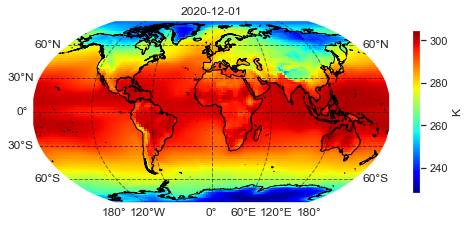
\includegraphics[width=\textwidth]{globe_sparse_full}
		\caption{Observed and unobserved data.}
	\end{subfigure}
	\hfill        
	\begin{subfigure}[b]{0.45\textwidth}
		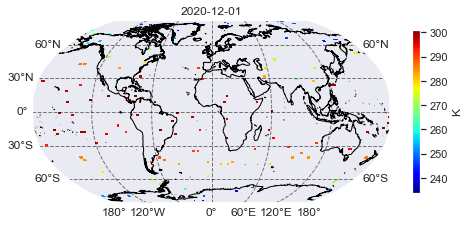
\includegraphics[width=\textwidth]{globe_sparse_train}
		\caption{Observed data.}
	\end{subfigure}
	\caption{An example of the sparsity induced from the  generating procedure in Section~\ref{ssec:cesm_globe} for the TREFHT variable of the CESM-LE dataset. Sparsity observed from the spatial view point.}
	\label{fig:cesm_sparsity}
\end{figure}

\subsection{European Study \label{ssec:cesm_eur}}
In contrast to the global study presented in Section~\ref{ssec:cesm_globe}, this study will consider a much narrower spatial domain.
We choose to observe in this study the domain bounded by the following latitude, longitude coordinates; $\left(-20, 35\right), \left(-20, 60\right), \left(45, 60\right), \left(-20, 60\right)$.
Here our spatial domain $\mathcal{S}$ is given by the following in latitude, longitude coordinate system; $\mathcal{S} = \left[-20, 45\right] \times \left[35, 60\right]$.
This corresponds roughly to European continent, and is indicated in Figure~\ref{fig:cesm_eur_bbox}.

\begin{figure}
	\centering
	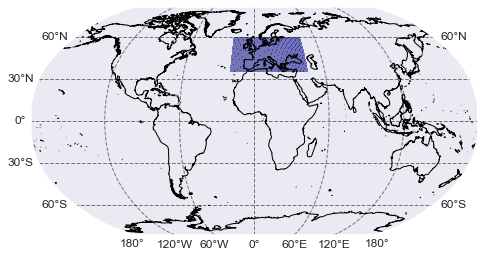
\includegraphics[width=\textwidth]{cesm_eur_bbox}
	\caption{Area of interest in the Europe study in blue. This is fixed and the same for each variable of interest in the CESM-LE dataset.}
	\label{fig:cesm_eur_bbox}
\end{figure}

The proposal of this study area is to consider a smaller spatial domain, where there is less likely to be large spatial variation. 
In this case we no longer downsample the resolution and keep the full resolution data from the CESM-LE datasets.
The study is then setup that we observe much more densely the functional data over this domain.
We use this setup to consider how well the CPACE framework deals with the intricacies of smaller scale variation as compared to the global study; which is designed to look at the frameworks ability to reconstruct functional data under for large scale variation.

Another difference we consider in this study is the frequency of observation.
In this study we choose to observe the functional data more regularly and at more locations across the domain.
Here this may be viewed as relating to the scenario of having many monitoring locations, but often readings are missing of your variable of interest due to technical difficulties.
For example, cloud obstructing imagery taken from satellites, \citep{meraner_cloud_2020}.
This sparsity is induced in our dataset for this study by using the following parameters to generate our training data.

We assume we observe $25\%$ of our possible spatial locations across our domain, $\mathcal{S}$.
As with our previous studies we further induce sparsity by assuming we only observe between $20\%$ and $40\%$ temporal points for each of these observations.
We do this independently for the $40$ simulations present in the CESM-LE dataset.
This construction is similar to that of the sparsity used in the simulation study in Section~\ref{sec:sim_study}.
These observed data we take to be our training data set.
The functional data which have partial observations on them we will take to be our validation data set.
The remaining unseen observations we take to be our test dataset for this study.
We do this process independently for each of the $40$ simulations present in the CESM-LE dataset.
Figure~\ref{fig:cesm_sparsity_eur} gives an indication of the training observations compared to the full data at a particular time point in the dataset for the TREFHT variable.
As can be seen this sparsity is less severe than that of the globe study, but still present.
We are interested mostly in this study as to whether the CPACE framework can help to reconstruct observations which vary on a smaller spatial scale.

\begin{figure}
	\centering
	\begin{subfigure}[b]{0.45\textwidth}
		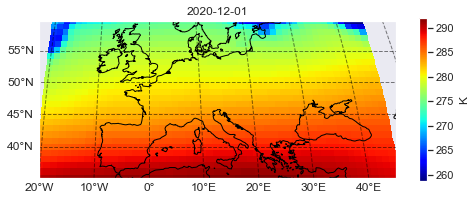
\includegraphics[width=\textwidth]{eur_sparse_full}
		\caption{Observed and unobserved data.}
	\end{subfigure}
	\hfill        
	\begin{subfigure}[b]{0.45\textwidth}
		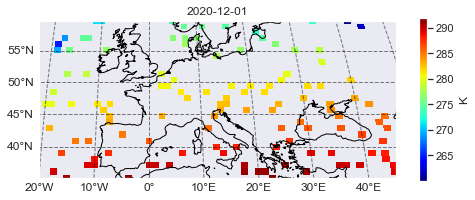
\includegraphics[width=\textwidth]{eur_sparse_train}
		\caption{Observed data.}
	\end{subfigure}
	\caption{An example of the sparsity induced from the  generating procedure in Section~\ref{ssec:cesm_eur} for the TREFHT variable of the CESM-LE dataset. Sparsity observed from the spatial view point.}
	\label{fig:cesm_sparsity_eur}
\end{figure}


\section{Spatial Kernels \label{sec:cesm_kernels}}
As in the simulation study from Section~\ref{sec:sim_study} we consider a variety of spatial kernels in the CPACE framework to compare to the FPCA approach.
In the following we describe the kernels which we use for the global and European study described in Section~\ref{sec:cesm_study}.
For most spatial kernels we must specify the metric between points of observation which captures the concept of distance in $\mathcal{S}$.
In all of our studies on the CESM-LE data we must consider how we define this for our domain $\mathcal{S}$ which as given is the surface of the globe.
We do so by projecting our domain from the surface of the globe to $\mathbb{R}^{3}$. 

\subsection{Domain Projection \label{ssec:spatial_projection}}
The coordinate system for the CESM-LE data is given in latitude and longitude.
The latitude of a point on the Earth's surface is the angle between the equatorial plane and the line which passes through that point and the centre of the Earth.
Similarly the longitude of a point on the Earth's surface is the angle between the prime meridian and another meridian which passes through that point. 
As such it describes a coordinate reference system (CRS) over the surface of the globe.
Therefore, when considering distance between two points in $\mathcal{S}$ we should consider the distance travelled on the globe between the two.
If the Earth was a true sphere this would be relatively simple as the distance between two points can be found using the great-circle distance.
This is given by the formula below for two points $\left(\text{lat}_1, \text{lon}_1\right)$ and $\left(\text{lat}_2, \text{lon}_2\right)$: 
\begin{equation}
	r \arccos\left(\sin(\text{lat}_1) \sin(\text{lat}_2) + \cos(\text{lat}_1) \cos(\text{lat}_2) \left( \text{lon}_1 - \text{lon}_2\right)\right)
\end{equation}

However, the world is not a true sphere and in fact a standard coordinate system which the CESM-LE data uses is the World Geodetic System (WGS) 84. 
This is a specific coordinate system which describes the surface of the globe using an ellipsoidal model, \citep{lu_geodetic_2014}. 
Thus the above great circle distance would be an approximation. 

Another issue with such an approach is how we define hyper parameters, such as length scale parameters in the Mat\'ern Three kernel (See Section~\ref{ssec:cesm_kern}), when using the WGS84 coordinate system.
Since the WGS84 defines the coordinate system using latitude and longitude it revolves around angles.
We would therefore need to consider sensible measure of distance between these angles which could have the added difficulty that period shifts shouldn't be further away.
Although possible, \citeauthor{guinness_isotropic_2016} discuss a variety in \citep{guinness_isotropic_2016}, they have computation complexities in implementing.

As such, and as suggested in \citep{guinness_isotropic_2016}, we decide to project our domain $\mathcal{S}$ into $\mathbb{R}^3$.
In this space we have alleviated the above issues as the standard concept of Euclidean distance will suffice in the kernels we study.
That is we project our surface of the globe into three dimensions, and calculate the distance between two points as the Euclidean distance in this space rather than using the great circle distance or a custom metric on the WGS84 coordinate system. 
Figure~\ref{fig:spatial_projection} highlights the difference between these approaches for the distance between two points on a circle and the euclidean distance.
Here we have reduced the dimension for ease of illustration but the same concept extends to three dimensions and the surface of the unit sphere. 

\begin{figure}[h]
	\centering
	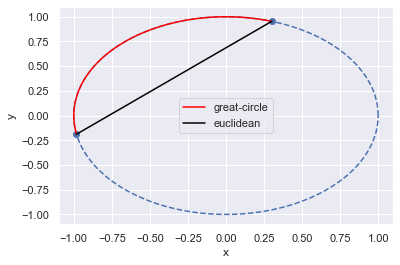
\includegraphics[width=\textwidth]{spatial_projection}
	\caption{Difference in great circle distance and the Euclidean distance in $\mathbb{R}^3$ for two points on the unit sphere.}
	\label{fig:spatial_projection}
\end{figure}

Although it is a simplification \citep{guinness_isotropic_2016} highlight it isn't a limiting factor, \citep{guinness_isotropic_2016}. 
Intuitively, this is because although our measure of distance between two points on the globe isn't accurate in the sense of true distance travelled our kernel hyper parameters will be estimated from the data and should allow for this from the observed correlation.
In particular the approach to projecting to $\mathbb{R}^3$ will overcome the issue of periodicity in using latitude and longitude systems.

Thus for each of the kernels specified below we first project our points in the spatial domain to $\mathbb{R}^3$ and then calculate the kernel value between them.
We use a projection from the WGS84 geodetic view of latitude, longitude to the geocentric view of element in $\mathbb{R}^3$, \citep{lu_geodetic_2014}, which corresponds to the projection that takes $\mathcal{S}$ from the surface of the globe to $\mathbb{R}^3$.

We do this for the full CPACE framework, for both likelihood calculation of our kernel hyper parameters and prediction.


\subsection{Kernels \label{ssec:cesm_kern}}
Our first kernel we consider is the White kernel, see Section~\ref{sssec:white_kern} for a complete description.
We will denote the CPACE model with this kernel as  \verb*|fpca_gp| in our studies as it corresponds to FPCA model which doesn't take into account the spatial dependency between functional observations but is estimated under our Gaussian process framework.

The second kernel we consider is the Anisotropic Mat\'ern Three kernel.
Alike in the simulation study, Section~\ref{sssec:matern_three}, this kernel follows a Mat\'ern form that is formed from specifying that $\nu=\frac{3}{2}$.
However in this kernel we let the length scale hyper parameter be different for each dimension of the domain.
That is the general form of the Anisotropic Mat\'ern Three kernel is given by:

\begin{equation}
	\zeta_k \left(\vesub{s}{i}, \vesub{s}{j}\right) = \lambda_k \left(1 + \sqrt{3}d \right)\exp \left(- \sqrt{3} d \right)
\end{equation}
where $d = \sqrt{\left(\vesub{s}{i} - \vesub{s}{j}\right) \vesup{R}{-1} \left(\vesub{s}{i} - \vesub{s}{j}\right)^\transpose}$, $R = \text{diag}\left(\ve{\rho}\right)$ and $\ve{\rho} = \left(\rho_1, \rho_2, \rho_3\right)^\transpose$ is our vector of length scale parameters per dimension.
Here we have restricted the anisotropy to a length scale over each dimension of the domain which is independent of each other by specifying the diagonal form of $R$.
In this case $R \in \mathbb{R}^{3 \times 3}$ as we will project our spatial domain to three dimensions as discussed in Section~\ref{ssec:spatial_projection}.
We will denote this kernel by \verb*|matern_three| for this study. 
Figure~\ref{fig:matern_aniso} highlights an example covariance structure using this anisotropic kernel with $\ve{\rho} = \left(1.0, 4.0, 4.0\right)$ on our spatial domain $\mathcal{S}$ projected.
Note the off diagonal structure which comes from the shorter length scale in the first dimension.
We choose to use an anisotropic stationary kernel, such as this, as it is well used in the literature for geospatial applications, \citep{cressie_statistics_2010}.
The anisotropy should allow the spatial kernel to capture difference in correlation between points of latitude and longitude which are often present in EO data sets. 

\begin{figure}[h]
	\centering
	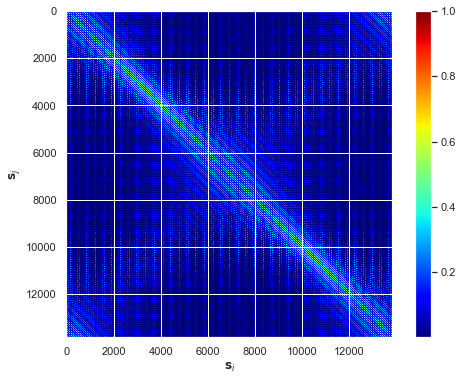
\includegraphics[width=\textwidth]{matern_aniso_ex}
	\caption{An example covariance structure with anisotropic Mat\'ern Three kernel.}
	\label{fig:matern_aniso}
\end{figure}

The final kernel we consider is the Gibbs kernel, \citep{gibbs_bayesian_1998}.
We use \verb*|gibbs| to denote this kernel in our studies.
This is similar to the one we utilised in the simulation study in Section~\ref{sssec:gibbs}. 
The only difference in the kernel we use for our study on the CESM-LE data is that we limit ourselves to two components in the kernels.
We do this after initial ad-hoc tries of differing number of components. 
We found that two components was more than enough to capture interesting components of the data whilst maintaining simple computation.
We speak more of this in Chapter~\ref{cha:implementation}.
Again, this is a non-stationary kernel which means it has the capability to capture non-stationary covariance structure in the CESM-LE dataset. 
Similarly, the construction of the kernel should also allow it to capture stationary covariance structures as well.
It also, alike the Mat\'ern Three kernel above should be able to capture any anisotropy in the data which is important for EO data, especially when observed at large spatial scales.

To compare the effectiveness of the CPACE models with different kernels and the FPCA framework we use a collection of metrics. 
We describe the metrics used in the study of the CESM-LE dataset in the following section. 

\section{Metrics \label{sec:metrics_cesm}}
Alike our simulation study, Section~\ref{sec:sim_study}, we use a variety of metrics to compare performance of our models.
As with the simulation study we consider the RMSE and MAE metrics on both the validation and test datasets separately.
These we consider are a measure of the ability of the models to reconstruct the individual pixel functions over the temporal domain.
The same reasoning as given in Section~\ref{sec:sim_study} is applicable for the choice of these metrics for evaluating model performance.

In addition to the RMSE and MAE metrics we also consider some metrics more tailored to image reconstruction.
We utilise the PSNR  and SSIM metrics, as described in Section~\ref{ssec:ftsm_sim_res}.
Both these metrics offer a comparison of perceived similarity between images.
This differs from the RMSE and MAE metrics which only consider difference between pixels in the images, and make no attempt to allow for the structure of the reconstruction.
We use these metrics as a further guage on the comparative performance of the CPACE framework with an eye to provide good reconstruction across the whole spatial domain.
As such, these metrics will be evaluated using the full dataset which is both the validation and test data combined. 
Both these metrics are also discussed in Section~\ref{ssec:ftsm_sim_res} and they're use in image reconstruction models is wide, \citep{hore_image_2010}.

We note as the CESM-LE data consists of $40$ replications of each variable of interest across our spatial-temporal domain, we can evaluate these metrics on each simulation and present the distribution of these metrics across the simulations.
We now proceed to discuss the results for both our globe and Europe study for each of our variables of interest from the CESM-LE dataset.

\section{Global Study Results \label{sec:cesm_res}}
Here we present the results of the study across the whole globe as described in Section~\ref{ssec:cesm_globe}.
We present the results separately for each variable of interest; Pressure (PS), Temperature (TREFHT), Precipitation (TMQ), and Wind Speed (U10).

We have considered four models for this study, the same setup for each variable of interest.
The \verb*|pace| model corresponds to the FPCA model or PACE framework, as describe in Chapter~\ref{cha:background},  which doesn't take into account spatial dependency.
The second, \verb*|fpca_gp|, is our CPACE model with the White kernel.
Again this doesn't take into account spatial dependency between functional observations, but is computed under our CPACE framework which allows for hyper parameters of the kernel; namely the spatial kernel variance for each components, to be estimated using the Gaussian process framework.
Thirdly, we use the Mat\'ern Three kernel with anisotropic length scales as the spatial kernel in another CPACE model.
This we denote by \verb*|matern_three|.
Finally, we denote by \verb*|gibbs| the CPACE model using the Gibbs kernel.
For each of these models we use $5$ components in our decomposition of the observed data which are applicable in both the PACE and CPACE framework. 

\subsection{Pressure\label{ssec:cesm_ps}}
Here we present and describe the results of using our CPACE framework to model the pressure variable from the CESM-LE dataset across the globe.

We begin by presenting the metric results for our validation data set.
These are reconstruction of partial observed functional data.
These are displayed in Table~\ref{tab:train_cesm_ps_globe}.
As can be seen there is a discrepancy between the CPACE models and the PACE model.
This can be seen as an impact of the large sparsity we have used in the study.
Since we assume such sparse observations it is obviously difficult for the FPCA model to truly capture the variations in the functional data.
This can be alleviated in the models which use spatial dependency as they can utilise spatial dependency to inform the curve at the prediction location to be similar to those close by.
It is alleviated in \verb*|fpca_gp| model since the CPACE framework allows for further estimation of the White kernel variances in accordance with the Gaussian process structure, something which the \verb*|pace| model doesn't allow for. 

\begin{table}
	\caption[Results for PS variable on validation data in the Global study]{Results for reconstruction of the validation data for the PS variable in the global study from the CESM-LE dataset. Bold indicates best in class. }
	\centering
	\label{tab:train_cesm_ps_globe}
	\begin{tabular}{lcc}
		\toprule
		\textbf{Model} & \textbf{RMSE} & \textbf{MAE} \\
		\midrule
		\verb*|pace| & 3634.1855 (2187.4974) & 1379.6860 (606.6431) \\
		\verb*|fpca_gp| & 726.3168 (129.7112)& 500.9342	(72.5722)\\
		\verb*|matern_three| & \textbf{629.5518	(83.7596)}& \textbf{454.7355	(45.9620)}\\
		\verb*|gibbs| & 704.5824 (100.7908) & 491.9828 (42.4173)\\
		\bottomrule
	\end{tabular}
\end{table}

We see this pattern again for the same metrics on the test data set.
These are presented in Table~\ref{tab:test_cesm_ps_globe}.
Again we can see the improvement resulting from the use of spatial information to help predict the curves.
We note the extremely poor performance of the \verb*|pace| model comes from a few simulations in the dataset having catastrophic errors.
The performance of this model on the other simulations is in line with the \verb*|fpca_gp| model.
We can see an illustration of this occurring in Figure~\ref{fig:train_ex_ps_globe}. 
Here we can see how the true curve is very variable, and although all our models get the relative shape of the curve, they completely miss the peaks and troughs.
This is because our component functions for these models haven't captured this aspect of the data.
This results in fairly large prediction errors.
However relative to the PACE framework our CPACE framework performs well.

In fact the Eigen decomposition is mostly dominated by the leading principal component.
This can be seen in Figure~\ref{fig:phi_ps_globe}.
This figure displays the effect of the first eigenfunction and the lighter grey curves show an example of the true functional data underlying.
As can be seen the models miss any periodic elements due to the fact that the major variation in this data comes from a shift in the curve level, which is captured in this eigenfunction. 


\begin{table}
	\caption[Results for PS variable on test data in the Global study]{Results for reconstruction of the test data for the PS variable in the global study from the CESM-LE dataset. Bold indicates best in class. Scale of $e+03$.}
	\centering
	\label{tab:test_cesm_ps_globe}
	\begin{tabular}{lcc}
		\toprule
		\textbf{Model} & \textbf{RMSE} & \textbf{MAE} \\
		\midrule
		\verb*|pace| & 4229.290 (298074.2) & 69.2113 (4.63648) \\
		\verb*|fpca_gp| & 12.4485	(2.9705) & 6.3486 (0.1641) \\
		\verb*|matern_three| & \textbf{2.5648 (0.0138)} & \textbf{1.3305 (0.0387)} \\
		\verb*|gibbs| & 3.8448 (0.6388) & 1.9998 (0.1129)\\
		\bottomrule
	\end{tabular}
\end{table}


\begin{figure}
	\centering
	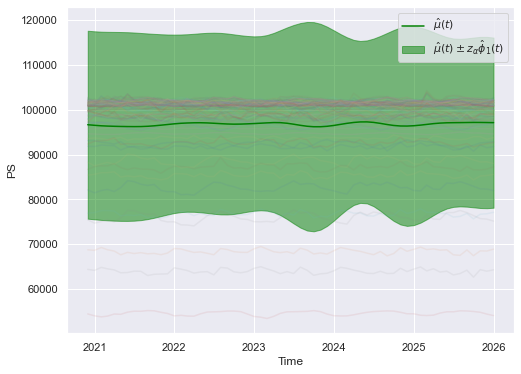
\includegraphics[width=\textwidth]{phi_ps_globe}
	\caption{The first eigenfunction from the FPCA decomposition used in all models for the PS variable in the global study.  Example true curves in light grey given for context.}
	\label{fig:phi_ps_globe}
\end{figure}

\begin{figure}
	\centering
	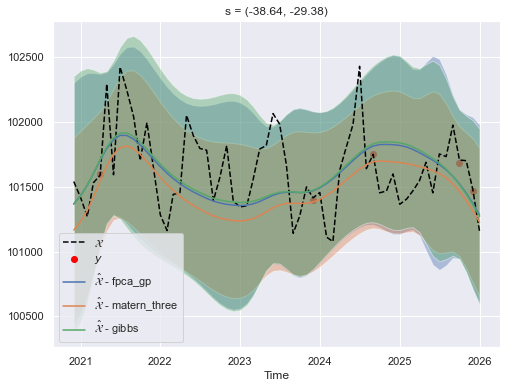
\includegraphics[width=\textwidth]{train_ex_ps_globe}
	\caption{An indicative example of the CPACE model performance on reconstruction of the CESM-LE Pressure variable from the validation dataset.}
	\label{fig:train_ex_ps_globe}
\end{figure}

Finally we consider the full dataset and present our image reconstruction metrics for this variable.
These are shown in Table~\ref{tab:full_cesm_ps_globe}.
Here we can clearly see the advantage of the Mat\'ern Three model over say the Gibbs model.
We can see a distinct advantage in both the PSNR and SSIM for this model.
We can also see a distinct advantage in using the CPACE methodology with the White kernel over the standard PACE methodology.
This is likely explainable due to the ability to fine tune the variance of the white kernels from the eigen decomposition. 
We illustrate further the comparative performances of these models by plotting the reconstruction for the dataset at a particular time point.
Figure~\ref{fig:full_ex_ps_globe} displays this.
We can see clearly the impact of utilising the spatial dependency but note we do fail to capture intricate details like the variance in pressure over South America.
Similarly we can see the Gibbs model captures some more intricate  spatial details but fails to match the Mat\'ern kernel in overall performance as it doesn't capture the scale of the changes as well. 

\begin{table}
	\caption[Results for PS variable on full data in the Globe study]{Results for reconstruction of the full data for the PS variable in the globe study from the CESM-LE dataset. Bold indicates best in class.}
	\centering
	\label{tab:full_cesm_ps_globe}
	\begin{tabular}{lcc}
		\toprule
		\textbf{Model} & \textbf{PSNR} & \textbf{SSIM} \\
		\midrule
		\verb*|pace| & -39.7596 (4.5310) & 0.4016	(0.0234) \\
		\verb*|fpca_gp| & 12.6672 (1.8675) & 0.4239 (0.0097) \\
		\verb*|matern_three| & \textbf{26.1533	(0.4736)} & \textbf{0.8364 (0.0068)}\\
		\verb*|gibbs| & 22.7488 (1.3351) & 0.7329	(0.0389)\\
		\bottomrule
	\end{tabular}
\end{table}

\begin{figure}
	\centering
	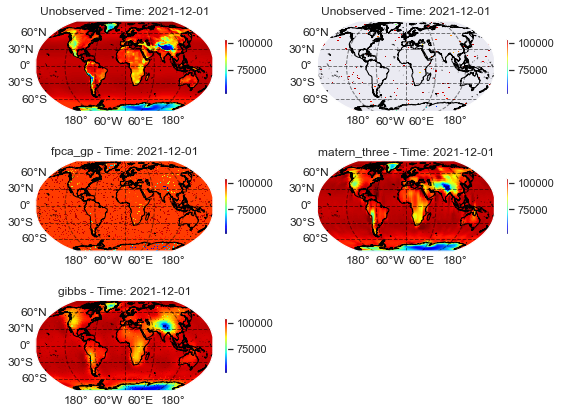
\includegraphics[width=\textwidth]{full_ex_ps_globe}
	\caption{An indicative example of the CPACE model performance on reconstruction for the full globe of the CESM-LE PS variable using the various models in the Global study. Clockwise from the top left we have the true data, the observed data at a particular time point, the Mat\'ern Three model reconstruction, the Gibbs model reconstruction, and the PACE model reconstruction under the CPACE framework.}
	\label{fig:full_ex_ps_globe}
\end{figure}

Overall, we can see that the CPACE framework adapts well to the pressure variable from the CESM-LE data set.
We can see from Figure~\ref{fig:phi_ps_globe} that we find an reasonable and interpretable eigenfunction, which corresponds to level shifts in the pressure.
However we find that this dominates the Eigen decomposition, and thus the results can have relatively large errors due to failing to capture intricate local variations in the data.
We view this as stemming from the sparsity of the study data set, as many of these variations are not observed in the training data.
For example, Figure~\ref{fig:train_ex_ps_globe} shows we only observe $2$ observations on that whole example function.
The CPACE models with spatial dependency perform drastically better for reconstruction from both the test metric perspective and the image reconstruction perspective. 
These promising results are a good indication of the usefulness of the CPACE framework with regards to EO data across the globe.

\subsection{Temperature \label{ssec:cesm_trefht}}
In this section we present and describe the results of using our CPACE framework to model the temperature variable from the CESM-LE dataset across the globe.
We present these in a similar way to Section~\ref{ssec:cesm_ps}.

In Table~\ref{tab:train_cesm_trefht_globe} we show the resulting metrics from the study on the validation dataset.
Here we can see again the distinct advantage of the CPACE framework and especially with using spatial dependency.
Similar to the Pressure variable results in Section~\ref{ssec:cesm_ps} we see that the Mat\'ern model performs best in class followed closely by the Gibbs model.

\begin{table}
	\caption[Results for TREFHT variable on validation data in the Global study]{Results for reconstruction of the validation data for the TREFHT variable in the global study from the CESM-LE dataset. Bold indicates best in class.}
	\centering
	\label{tab:train_cesm_trefht_globe}
	\begin{tabular}{lcc}
		\toprule
		\textbf{Model} & \textbf{RMSE} & \textbf{MAE} \\
		\midrule
		\verb*|pace| & 8.2170	(0.2680) & 5.5581 (0.1505) \\
		\verb*|fpca_gp| & 7.9646	(0.1809) & 5.4940 (0.1154) \\
		\verb*|matern_three| & \textbf{7.3703 (0.1805)}& \textbf{5.2337 (0.1198)}\\
		\verb*|gibbs| & 7.7548 (0.7118) & 5.4087 (0.1170)\\
		\bottomrule
	\end{tabular}
\end{table}

Next we consider the test reconstructions.
That is reconstruction of completely unobserved functions. 
An example of such reconstructions for our models considered is given in Figure~\ref{fig:test_ex_trefht_globe}.

\begin{figure}
	\centering
	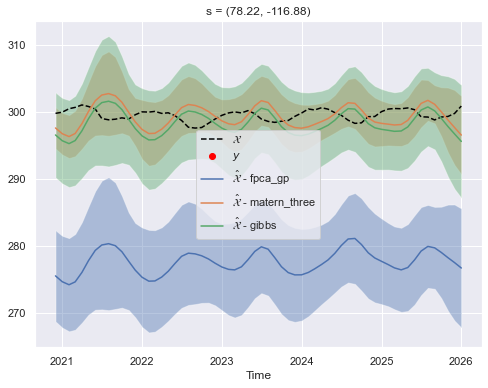
\includegraphics[width=\textwidth]{test_ex_trefht_globe}
	\caption{An indicative example of the CPACE model performance on reconstruction of the CESM-LE TREFHT variable in the global study from the test dataset.}
	\label{fig:test_ex_trefht_globe}
\end{figure}

Here we can clearly see the impact of using the spatial dependency which has the main advantage of being able to pick out the correct level shift of the mean function to match that of the unobserved functional data. 
We can also see that the Mat\'ern kernel has a tighter confidence band than that of the Gibbs model, which may be a bit of an over estimate coming from model mis-specification, since the true curve sometimes falls outside this band, whereas with the Gibbs kernel  it does not. 
The full metric results for the test data are given in Table~\ref{tab:test_cesm_trefht_globe}. 
This indicates that the Mat\'ern model is the best in class for the test data albeit within the range of the Gibbs model's performance. 
Noting this, one may well choose to prefer the Gibbs model.
However, yet again we see that either of these models are vastly superior to the others.

This is confirmed if we consider the image reconstruction metrics for this dataset.
In Table~\ref{tab:full_cesm_trefht_globe} we can see clearly the difference in terms of image similarity between reconstructions under the various models. 
For illustration, we display an example reconstruction using the various models in Figure~\ref{fig:full_ex_trefht_globe}.

\begin{table}
	\caption[Results for TREFHT variable on test data in the Global study]{Results for reconstruction of the test data for the TREFHT variable in the global study from the CESM-LE dataset. Bold indicates best in class.}
	\centering
	\label{tab:test_cesm_trefht_globe}
	\begin{tabular}{lcc}
		\toprule
		\textbf{Model} & \textbf{RMSE} & \textbf{MAE} \\
		\midrule
		\verb*|pace| & 23.3642	(1.7618) & 17.9309 (0.2215) \\
		\verb*|fpca_gp| & 22.2936	(0.1841) & 17.8549 (0.1656) \\
		\verb*|matern_three| & \textbf{7.5008 (0.1373)}& \textbf{5.2875 (0.1387)}\\
		\verb*|gibbs| & 7.8361 (0.0916) & 5.7924 (0.0855)\\
		\bottomrule
	\end{tabular}
\end{table}

\begin{table}
	\caption[Results for TREFHT variable on full data in the Global study]{Results for reconstruction of the full data for the TREFHT variable in the globe study from the CESM-LE dataset. Bold indicates best in class.}
	\centering
	\label{tab:full_cesm_trefht_globe}
	\begin{tabular}{lcc}
		\toprule
		\textbf{Model} & \textbf{PSNR} & \textbf{SSIM} \\
		\midrule
		\verb*|pace| & 12.2512 (0.6205) & 0.2634	(0.0043) \\
		\verb*|fpca_gp| & 12.6409 (0.0749) & 0.2668 (0.0036) \\
		\verb*|matern_three| & \textbf{22.5449	(0.2070)} & \textbf{0.8216 (0.0037)}\\
		\verb*|gibbs| & 21.9926 (0.2059) & 0.7965	(0.0092)\\
		\bottomrule
	\end{tabular}
\end{table}

\begin{figure}
	\centering
	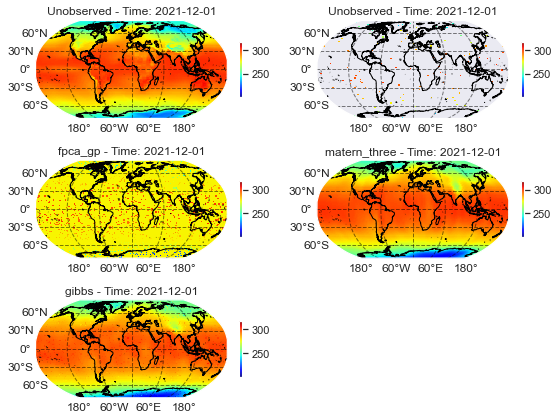
\includegraphics[width=\textwidth]{full_ex_trefht_globe}
	\caption{An indicative example of the CPACE model performance on reconstruction for the full globe of the CESM-LE TREFHT variable using the various models in the global study. Clockwise from the top left we have the true data, the observed data at a particular time point, the Mat\'ern Three model reconstruction, the Gibbs model reconstruction, and the PACE model reconstruction under the CPACE framework.}
	\label{fig:full_ex_trefht_globe}
\end{figure}

Alike Section~\ref{ssec:cesm_ps}, we find similar patterns in our study.
The CPACE framework outperforms the PACE methodology but we don't manage to truly capture all underlying eigenfunctions from our dataset.
Again as our study is using extremely sparse data this is understandable, as we simply haven't seen this variation in the training data.
For the temperature variable the Mat\'ern model tends to perform best however the Gibbs models is in close competition, and often may perform better with a more useful confidence level.
In fact Figure~\ref{fig:cesm_trefht_dist} highlight this by showing that the SSIM metric for the Gibbs kernel can outperform the Mat\'ern model; just not on average.
This may be because, in certain scenarios, the Gibbs kernel with its extra hyper parameters fails to converge to the best solution. 
Occasionally it will, and in those scenarios will capture more of the complex nature of the spatial dependency. 

\begin{figure}
	\centering
	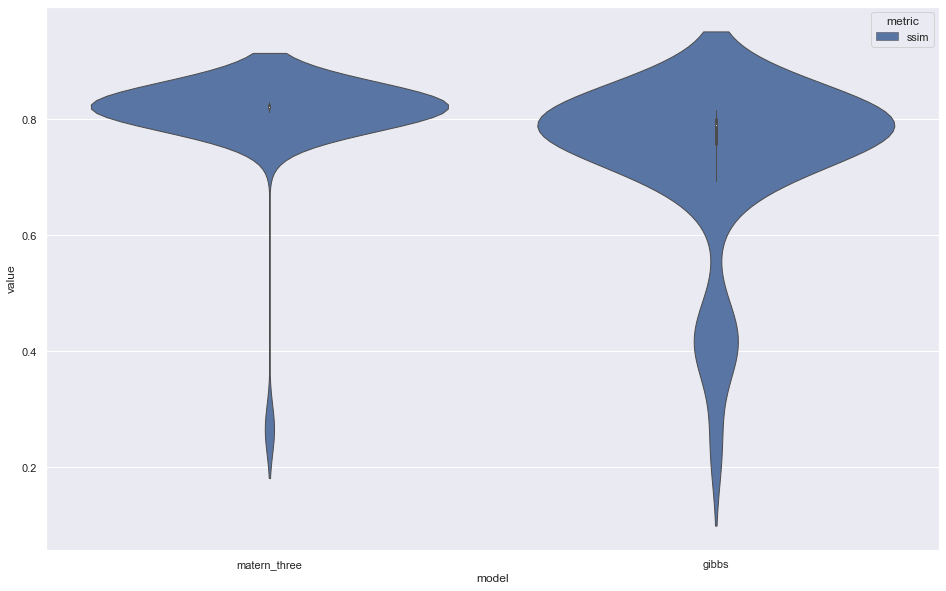
\includegraphics[width=\textwidth]{cesm_trefht_dist}
	\caption{Distribution plot of the SSIM metric for the Gibbs and Mat\'ern kernel models for the TREFHT variable.}
	\label{fig:cesm_trefht_dist}
\end{figure}

\subsection{Precipitation \label{ssec:cesm_tmq}}
In this section we present the results of the global study for the precipitation variable, TMQ.
We start by considering the decomposition of the data. 

One important aspect of both the PACE and CPACE methodologies is the Eigen decomposition of the data common to both. 
Figure~\ref{fig:phi_tmq_globe} shows the impact of the first two eigenfunctions in the FPCA decomposition.
We can see from the first eigenfunction, Figure~\ref{fig:phi_1_tmq_globe}, that this clearly represents a level shift in the functions.
This is similar to the first eigenfunction from the study on the PS variable.
This intuitively makes sense as we would expect different base precipitation level for different areas of the globe.
The second eigenfunction, Figure~\ref{fig:phi_2_tmq_globe}, is perhaps a bit more complicated.
This can be considered as an eigenfunction which will stretch the peaks and troughs of the mean function.
These eigenfunctions are encouraging as it suggest that both the PACE and CPACE frameworks are appropriate for this dataset as they are outputting eigenfunctions with relatable interpretations.
We note as with the study on the PS variable that the first eigenfunction is particularly dominating.
This again is understandable as we can see that the main mode of variation comes from a level shift.
However, it is disappointing that the second eigenfunction doesn't pick up the drastic changes in peaks that are present in some locations. 
This is most likely due to the sparsity of observations used for training meaning it isn't obviously present from the training data only.

\begin{figure}
	\centering
	\begin{subfigure}[b]{0.45\textwidth}
		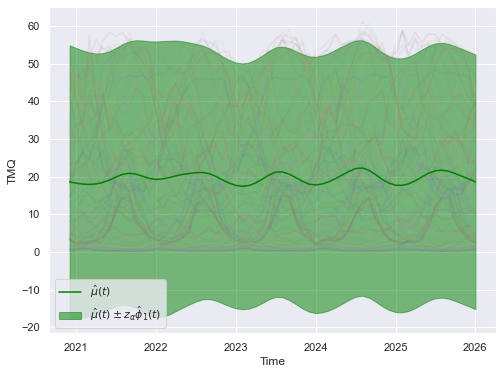
\includegraphics[width=\textwidth]{phi_1_tmq_globe}
		\caption{First eigenfunction.}
		\label{fig:phi_1_tmq_globe}
	\end{subfigure}
	\hfill        
	\begin{subfigure}[b]{0.45\textwidth}
		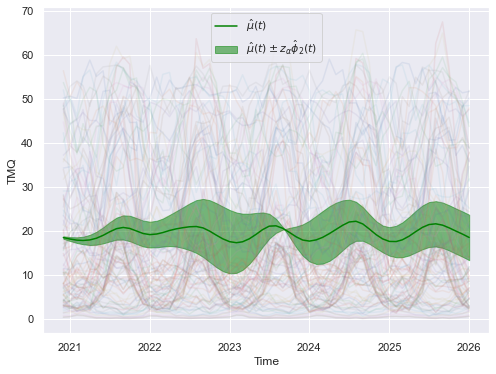
\includegraphics[width=\textwidth]{phi_2_tmq_globe}
		\caption{Second eigenfunction.}
		\label{fig:phi_2_tmq_globe}
	\end{subfigure}
	\caption{The first two eigenfunctions impact on the mean function from the PACE and CPACE framework of the TMQ variable in the global study. Here the shaded region shows the impact of two standard deviations from the mean function using the corresponding eigenfunction. Sample curves from the dataset are plotted for context.}
	\label{fig:phi_tmq_globe}
\end{figure}

Next we consider the ability for our models to reconstruct observed and unobserved data. 
Table~\ref{tab:train_cesm_tmq_globe} displays the metrics for the partially observed validation data reconstruction and Table~\ref{tab:test_cesm_tmq_globe} displays the metrics for the unobserved test data reconstruction.
It is interesting to note that the Gibbs model provides best in class performance on the  validation data.
We can also see, similarly to that study, that the Mat\'ern model performs best in class for the test data, while the Gibbs model performs close to best in class.
The Gibbs model's test metrics have a much larger variance, and suggest that while it performs on average worse than the Mat\'ern model it occasionally may produce better results.
This is probably an effect of over fitting the complex non-stationary model which underpins the Gibb's model.
Whereas the Mat\'ern model has a relatively simpler kernel, and thus estimating its hyper parameters is less prone to error.

\begin{table}
	\caption[Results for TMQ variable on training data in the Global study]{Results for reconstruction of the training data for the TMQ variable in the global study from the CESM-LE dataset. Bold indicates best in class.}
	\centering
	\label{tab:train_cesm_tmq_globe}
	\begin{tabular}{lcc}
		\toprule
		\textbf{Model} & \textbf{RMSE} & \textbf{MAE} \\
		\midrule
		\verb*|pace| & 6.3678 (0.1285) & 4.5960 (0.0765) \\
		\verb*|fpca_gp| & 6.2901	(0.0902) & 4.5786 (0.0779) \\
		\verb*|matern_three| & 5.5912 (0.2185)& 4.1445 (0.1806)\\
		\verb*|gibbs| & \textbf{5.1159 (0.2066)} & \textbf{3.7297 (0.1773)}\\
		\bottomrule
	\end{tabular}
\end{table}

\begin{table}
	\caption[Results for TMQ variable on test data in the Global study]{Results for reconstruction of the test data for the TMQ variable in the global study from the CESM-LE dataset. Bold indicates best in class.}
	\centering
	\label{tab:test_cesm_tmq_globe}
	\begin{tabular}{lcc}
		\toprule
		\textbf{Model} & \textbf{RMSE} & \textbf{MAE} \\
		\midrule
		\verb*|pace| & 15.8224 (0.0925) & 13.0445 (0.0824) \\
		\verb*|fpca_gp| & 15.7821 (	0.0643) & 13.0326 (0.0760) \\
		\verb*|matern_three| & \textbf{6.1061 (0.0778)}& \textbf{4.4798 (0.0522)}\\
		\verb*|gibbs| & 6.3401 (0.0934) & 4.7312 (0.0715)\\
		\bottomrule
	\end{tabular}
\end{table}

An illustration of the reconstruction ability from the temporal point of view for test data is given in Figure~\ref{fig:test_ex_tmq_globe}.
It highlights the improvement that the spatial models can make, but also points out that we are not capturing truly the underlying functions.
It is evident that we clearly miss the change in periodicity of the curves.
Again this may be difficult to pick up based on the sparsity of our observed data.
The sparsity of observations can be seen from Figure~\ref{fig:full_ex_tmq_globe} which gives an illustration of the reconstruction ability spatially.
This figure also highlights the discrepancy between the Gibbs and the Mat\'ern model.
We can see that the Gibbs model although has some areas of correct structure fails to capture fully the data across the whole domain, whereas the Mat\'ern model achieves a much better global structure.

\begin{figure}
	\centering
	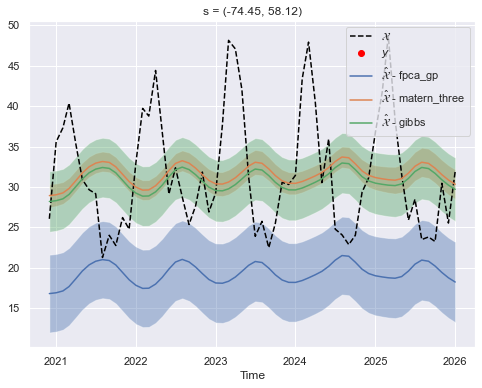
\includegraphics[width=\textwidth]{test_ex_tmq_globe}
	\caption{Example reconstruction for unobserved curves between our studied models.}
	\label{fig:test_ex_tmq_globe}
\end{figure}

\begin{figure}
	\centering
	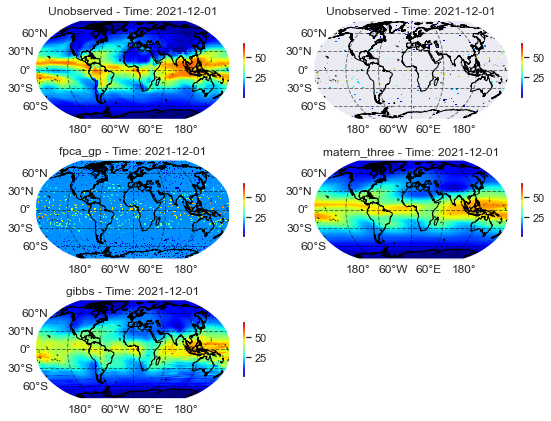
\includegraphics[width=\textwidth]{full_ex_tmq_globe}
	\caption{An indicative example of the CPACE model performance on reconstruction for the full globe of the CESM-LE TMQ variable using the various models in the global study. Clockwise from the top left we have the true data, the observed data at a particular time point, the Mat\'ern Three model reconstruction, the Gibbs model reconstruction, and the PACE model reconstruction under the CPACE framework.}
	\label{fig:full_ex_tmq_globe}
\end{figure}


\subsection{Wind Speed\label{ssec:cesm_u10}}
We present the results of the global study for the wind speed variable, U10.
Similar to the other global studies we focus on the training and test metrics.

First, the training metrics.
These are displayed in Table~\ref{tab:train_cesm_u10_globe}.
We can see that on the training data models perform similarly well, with the Mat\'ern and Gibbs models performing best in class.
However all models seem to have similar reconstruction ability.
We can see an illustration of the relative performances of the models on training data in Figure~\ref{fig:train_ex_u10_globe}.
This also identifies that we seem to have missed again the periodicity in the model.
Again, similar to the previous variables, this is down to the models focusing on the level shift as their main mode of variation.

\begin{table}
	\caption[Results for U10 variable on validation data in the Globe study]{Results for reconstruction of the validation data for the U10 variable in the globe study from the CESM-LE dataset. Bold indicates best in class.}
	\centering
	\label{tab:train_cesm_u10_globe}
	\begin{tabular}{lcc}
		\toprule
		\textbf{Model} & \textbf{RMSE} & \textbf{MAE} \\
		\midrule
		\verb*|pace| & 1.2952 (0.0153) & 0.9343	(0.0163) \\
		\verb*|fpca_gp| & 1.2879 (0.0121) & 0.9306 (0.0120) \\
		\verb*|matern_three| & \textbf{1.2659 (0.0106)}& 0.9343	(0.0107)\\
		\verb*|gibbs| & 1.2761	(0.0135) & \textbf{0.9215	(0.0095)}\\
		\bottomrule
	\end{tabular}
\end{table}

\begin{figure}
\centering
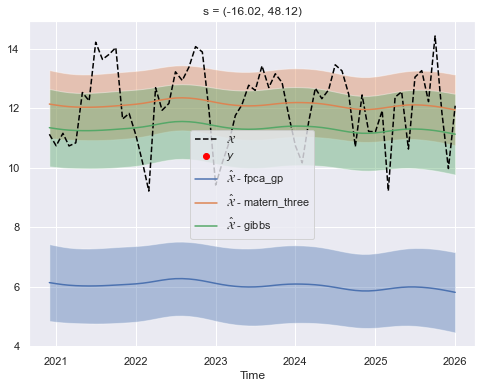
\includegraphics[width=\textwidth]{test_ex_u10_globe}
\caption{Example reconstruction for partially observed curves between our studied models.}
\label{fig:train_ex_u10_globe}
\end{figure}

We next consider the test data performance, and display the metrics for this in Table~\ref{tab:test_cesm_u10_globe}.
We can see a clear distinction in the test metrics in preference to the CPACE models with the spatial kernels.
It seems that the simpler Mat\'ern model is performing best over all.
However the distinction between that and the Gibbs model is small from these metrics.
Considering our image reconstruction metrics, we can see a clearer preference to the Mat\'ern model, see Table~\ref{tab:full_cesm_u10_globe}. 
It is interesting to note that the Gibbs model can outperform that of the Mat\'ern model in certain situations.
We can see this by looking at the distribution of them SSIM metric over the simulations present in the CESM-LE dataset for the global study.
We show this in Figure~\ref{fig:cesm_u10_dist}, where the distribution of the \verb*|gibbs| model metrics has a higher peak SSIM. 
However, over all simulations, we also see a larger range which is on average lower than the \verb*|matern_three| model. 
Hence, the poorer performance on average.


\begin{table}
	\caption[Results for U10 variable on test data in the Global study]{Results for reconstruction of the training data for the U10 variable in the global study from the CESM-LE dataset. Bold indicates best in class.}
	\centering
	\label{tab:test_cesm_u10_globe}
	\begin{tabular}{lcc}
		\toprule
		\textbf{Model} & \textbf{RMSE} & \textbf{MAE} \\
		\midrule
		\verb*|pace| & 3.0124 (0.0107) & 2.5004	(0.0103) \\
		\verb*|fpca_gp| & 3.0098 (0.0116) & 2.4991 (0.0103) \\
		\verb*|matern_three| & \textbf{1.4713 (0.0129)}& \textbf{1.0965	(0.0128)}\\
		\verb*|gibbs| & 1.5642	(0.0318) & 1.2051	(0.0125)\\
		\bottomrule
	\end{tabular}
\end{table}

\begin{table}
	\caption[Results for U10 variable on training data in the Global study]{Results for reconstruction of the test data for the U10 variable in the global study from the CESM-LE dataset. Bold indicates best in class.}
	\centering
	\label{tab:full_cesm_u10_globe}
	\begin{tabular}{lcc}
		\toprule
		\textbf{Model} & \textbf{PSNR} & \textbf{SSIM} \\
		\midrule
		\verb*|pace| & 13.7495	(0.0743) & 0.1699 (0.0021) \\
		\verb*|fpca_gp| & 13.7673 (0.0669)& 0.1703 (0.0021) \\
		\verb*|matern_three| & \textbf{19.8017 (0.0731)}& \textbf{0.5988 (0.0092)}\\
		\verb*|gibbs| & 19.2793	(0.1095) & 0.5230 (0.0089)\\
		\bottomrule
	\end{tabular}
\end{table}

\begin{figure}
	\centering
	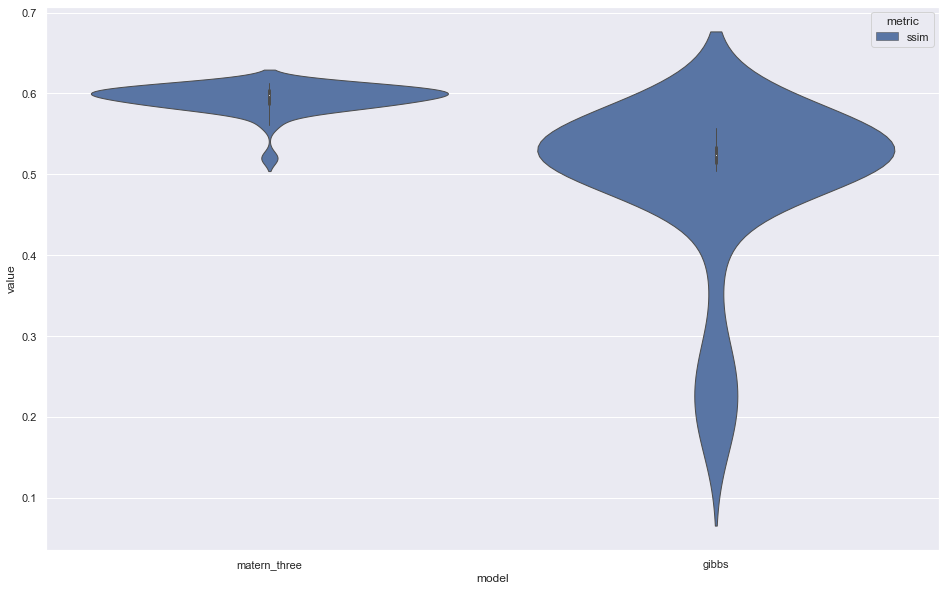
\includegraphics[width=\textwidth]{cesm_u10_dist}
	\caption{Distribution plot of the SSIM metric for the Gibbs and Mat\'ern kernel models for the U10 variable from the global study.}
	\label{fig:cesm_u10_dist}
\end{figure}

Finally, we provide an indicative reconstruction over both a spatial view, see Figure~\ref{fig:full_ex_u10_globe}, and a temporal view, see Figure~\ref{fig:test_ex_u10_globe}.
We can see from these that we have some limitation in our ability to reconstruct the periodic components of the functional observations.
As mentioned before, this is likely because we just don't have enough evidence from our training data to suggest such periodic components in our FPCA decomposition which all models use.

\begin{figure}
\centering
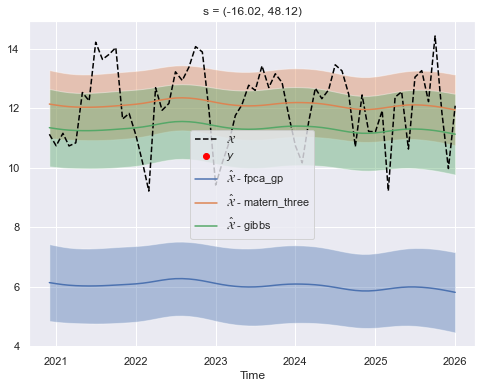
\includegraphics[width=\textwidth]{test_ex_u10_globe}
\caption{Example reconstruction for unobserved curves between our studied models for the U10 variable in the global study.}
\label{fig:test_ex_u10_globe}
\end{figure}

\begin{figure}
\centering
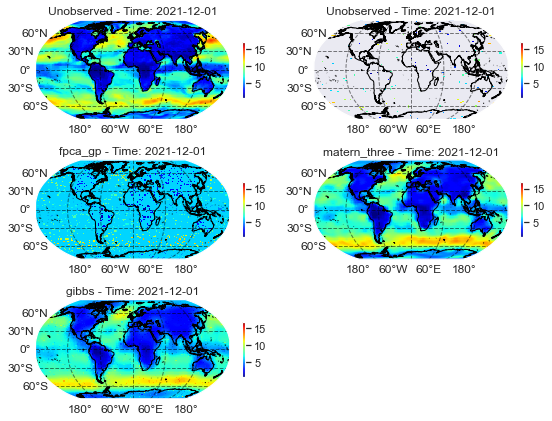
\includegraphics[width=\textwidth]{full_ex_u10_globe}
\caption{An indicative example of the CPACE model performance on reconstruction for the full globe of the CESM-LE U10 variable using the various models in the global study. Clockwise from the top left we have the true data, the observed data at a particular time point, the Mat\'ern Three model reconstruction, the Gibbs model reconstruction, and the PACE model reconstruction under the CPACE framework.}
\label{fig:full_ex_u10_globe}
\end{figure}

\subsection{Discussion \label{ssec:globe_discussion}}
In Sections~\ref{ssec:cesm_ps},~\ref{ssec:cesm_trefht},~\ref{ssec:cesm_tmq},~\ref{ssec:cesm_u10} we have considered an application of the CPACE model to the global study of the CESM-LE data. 
We have presented results which show clearly the advantage of using the CPACE framework with spatial kernels.
This is intuitive as the geographic nature of this dataset clearly should have spatial dependency for all of these variables.

Our results presented show that typically the Mat\'ern model tends to perform best out of our models considered.
This is intriguing since we may expect the non-stationary component of the Gibbs model to pick out perhaps more complex spatial dependencies.
We suppose the reason for the lack of this is two fold.
Firstly; on the global scale, with our reduced resolution we may indeed mask a lot of these complexities, since the variation across large spatial scales dwarfs the subtleties of local variation.
Secondly; our challenge of using sparse training data for this study may have meant that we often exclude a lot of intricate variation by simply not having enough evidence in the training datasets. 
This theory is backed up by the fact that in the most case the Gibbs kernel tends itself towards behaving like the Mat\'ern kernel.
This is comforting as it suggest that rather than the Gibbs model failing to identify these trends, it is actually that our training data only suggests large scale variation.

We also note that in the study across the variables our eigen decomposition which makes the base of all these models tended to be dominated by a single large component.
This represented a level shift of the functional data.
The CPACE models with a spatial kernel tend to outperform the other as they use spatial information to inform on where to apply this level shift.
This leads to a good increase in performance.
Again, this intuitively makes sense which gives us comfort in the feasibility of the CPACE framework being applied to EO data as it produces interpretable results.

We note that even in the non-spatial dependent kernels the CPACE framework tends to outperform the PACE framework.
Again, attributable to the additional refinement of the models hyper parameters compared to the PACE model.

In the following section we move on to consider our European study. 
This more localised European study, presented in Section~\ref{ssec:cesm_eur}, will consider a slightly different challenge to the CPACE framework with less sparse data and less global variation.

\section{European Study Results \label{sec:cesm_res_eurr}}
Here we present the results of the study across the spatial domain as described in Section~\ref{ssec:cesm_eur}.
This roughly corresponds to the European continent.
This study has two components that differ from the global study; namely the spatial scale and the density of observations.
This gives us a chance to see how well the CPACE framework compares to the PACE framework under these scenarios.

We have considered four models for this study, the same setup for each variable of interest.
The \verb*|fpca| model corresponds to the FPCA model or PACE framework, which doesn't take into account spatial dependency.
The second, \verb*|fpca_gp|, is our CPACE model with the White kernel.
Again this doesn't take into account spatial dependency between functional observations, but is computed under our CPACE framework which allows for hyper parameters of the kernel; namely the spatial kernel variance for each components, to be estimated using the Gaussian process framework.
Thirdly, we use the Mat\'ern Three kernel with anisotropic length scales as the spatial kernel in another CPACE model.
This we denote by \verb*|matern_three|.
Finally, we denote by \verb*|gibbs| the CPACE model using the Gibbs kernel.
For each of these models we use $5$ components in our decomposition of the observed data and in the CPACE framework. 

We present the results separately for each variable of interest; Pressure (PS), Temperature (TREFHT), Precipitation (TMQ), and Wind Speed (U10).

\subsection{Pressure \label{ssec:cesm_ps_eur}}
Here we present the results from our models applied to the Pressure variable in the European study.
We start by looking at the eigen decomposition common to all models.
Figure~\ref{fig:phi_ps_eur} displays the impact of the first two eigen functions under this study for a single simulation of the PS variable from the CESM-LE dataset.
It is of note that again the first eigenfunction, Figure~\ref{fig:phi_1_ps_eur}, represents a level shift; as was seen in the global study of the pressure variable.
The second eigenfunction, Figure~\ref{fig:phi_2_ps_eur}, shows this time however a stretching of the peaks and troughs from the mean function.
It is perhaps slightly more complicated that that,  showing more variation at the start and end of the domain, but in general that is a fair interpretation of the second eigenfunction.
This is encouraging as intuitively this is an important part of the data set and highlights the ability of the PACE methodology to help in understanding the data, something which the CPACE methodology builds on.
It is also interesting to note that we obtain a much more representative mean function than that of the global study.
This is a result of the denser observations and the smaller spatial scale in this study.

\begin{figure}
	\centering
	\begin{subfigure}[b]{0.45\textwidth}
		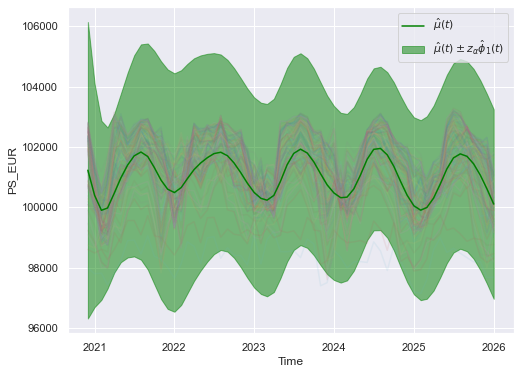
\includegraphics[width=\textwidth]{phi_1_ps_eur}
		\caption{First eigenfunction.}
		\label{fig:phi_1_ps_eur}
	\end{subfigure}
	\hfill        
	\begin{subfigure}[b]{0.45\textwidth}
		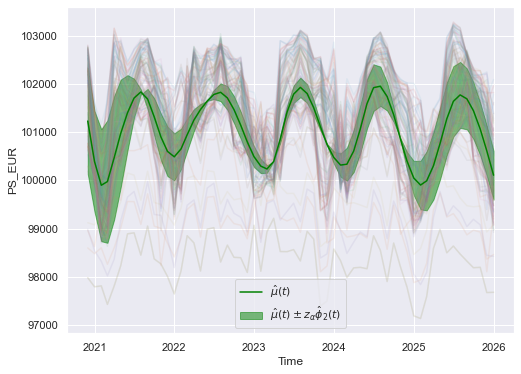
\includegraphics[width=\textwidth]{phi_2_ps_eur}
		\caption{Second eigenfunction.}
		\label{fig:phi_2_ps_eur}
	\end{subfigure}
	\caption{The first two eigenfunctions impact on the mean function from the PACE and CPACE framework for the PS variable in the European study. Here the shaded region shows the impact of two standard deviations from the mean function using the corresponding eigenfunction. Sample curves from the dataset are plotted for context.}
	\label{fig:phi_ps_eur}
\end{figure}

Next we present the metrics of the predictions from our variety of models.
We start by showing the resultant metrics on our validation data set in Table~\ref{tab:train_cesm_ps_eur}.
Again, similar to the global study we see a close comparative performance between all models.
All models perform roughly equally on the validation data set.
Perhaps we argue that the spatial models perform slightly better than the non-spatial models, especially evident on the MAE metric.
An indicative example of model reconstruction is given in Figure~\ref{fig:train_ex_ps_eur}.
It highlights how similar the models predict partially observed functions. 

\begin{table}
	\caption[Results for PS variable on validation data in the European study]{Results for reconstruction of the validation data for the PS variable in the European study from the CESM-LE dataset. Bold indicates best in class.}
	\centering
	\label{tab:train_cesm_ps_eur}
	\begin{tabular}{lcc}
		\toprule
		\textbf{Model} & \textbf{RMSE} & \textbf{MAE} \\
		\midrule
		\verb*|pace| & 579.4300 (47.2497) & 438.0766 (28.8890) \\
		\verb*|fpca_gp| & 562.3507 (38.1133) & 431.3178 (27.2087) \\
		\verb*|matern_three| & 560.6262 (41.2007)& \textbf{423.1480 (27.5427)}\\
		\verb*|gibbs| & 559.1836 (36.0552) & 424.4744 (25.5373)\\
		\bottomrule
	\end{tabular}
\end{table}

\begin{figure}
	\centering
	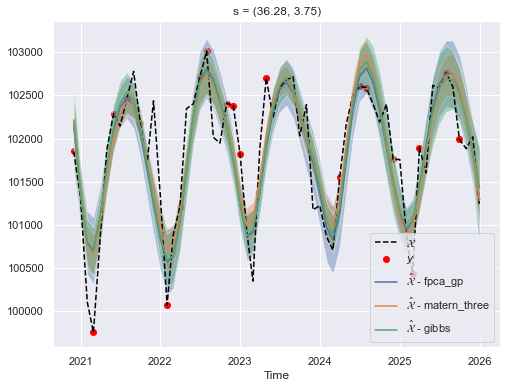
\includegraphics[width=\textwidth]{train_ex_ps_eur}
	\caption{Example reconstruction for partially observed curves between our studied models for the PS variable in the European study.}
	\label{fig:train_ex_ps_eur}
\end{figure}

Next we consider the performance on the test dataset, that is completely unobserved functional data.
We present the metric results for this in Table~\ref{tab:test_cesm_ps_eur}.
As can be seen, we see a distinct improvement in using the CPACE framework with a spatial kernel.
The Mat\'ern kernel performs best in class.
The Gibbs kernel unfortunately suffers from occasional bad prediction accuracy on some simulations leading to higher metric results with larger variance.
This is probably due to the added complexity in estimating the kernel hyper parameters.
We discuss our approach to minimising this effect in Chapter~\ref{cha:implementation}.

\begin{table}
	\caption[Results for PS variable on test data in the European study]{Results for reconstruction of the test data for the PS variable in the European study from the CESM-LE dataset. Bold indicates best in class.}
	\centering
	\label{tab:test_cesm_ps_eur}
	\begin{tabular}{lcc}
		\toprule
		\textbf{Model} & \textbf{RMSE} & \textbf{MAE} \\
		\midrule
		\verb*|pace| & 1297.1985 (29.4383) & 760.5791 (12.6591) \\
		\verb*|fpca_gp| & 1297.1985 (29.4383) & 760.5791 (12.6591) \\
		\verb*|matern_three| & \textbf{667.1006 (64.2558)}& \textbf{465.4720 (24.7951)}\\
		\verb*|gibbs| & 942.3990 (125.7554) & 532.5312 (25.7204)\\
		\bottomrule
	\end{tabular}
\end{table}

An example reconstruction from these models for an functional data from the test set is displayed in Figure~\ref{fig:test_ex_ps_eur}. 
This shows how the spatial models can adapt using the location of the spatial domain, whereas the non-spatial dependent kernel will just predict the mean function.

\begin{figure}
	\centering
	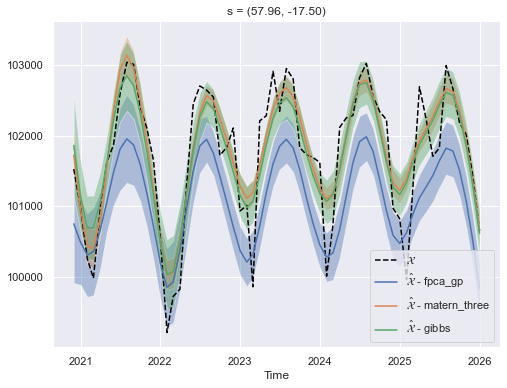
\includegraphics[width=\textwidth]{test_ex_ps_eur}
	\caption{Example reconstruction for unobserved curves between our studied models for the PS variable in the European study.}
	\label{fig:test_ex_ps_eur}
\end{figure}

Finally we consider the image reconstruction metrics.
These consider how well the models perform to recreate the imagery as a whole. 
This is presented in Table~\ref{tab:full_cesm_ps_eur}.
Again, we can see the better performance of the spatial kernels, with the Mat\'ern kernel quite expectedly being best in class.
Interestingly, the performance increase over the non-spatial kernel models is less pronounced than in the global study.
This is a function of the less varied data and the increase in observations, which gives the non-spatial models more points at which the functions have some observations which is where they perform best.

\begin{table}
	\caption[Results for PS variable on full data in the European study]{Results for reconstruction of the full data for the PS variable in the European study from the CESM-LE dataset. Bold indicates best in class.}
	\centering
	\label{tab:full_cesm_ps_eur}
	\begin{tabular}{lcc}
		\toprule
		\textbf{Model} & \textbf{PSNR} & \textbf{SSIM} \\
		\midrule
		\verb*|pace| & 21.6920 (0.1913) & 0.7137 (0.0121) \\
		\verb*|fpca_gp| & 21.6992 (0.1913)& 0.7246	(0.0086) \\
		\verb*|matern_three| & \textbf{27.2527	(0.8316)}& \textbf{0.8947 (0.0130)}\\
		\verb*|gibbs| & 23.8517	(1.4678) & 0.8655 (0.0168)\\
		\bottomrule
	\end{tabular}
\end{table}

From the above, we can see clear evidence that the CPACE framework is effective for the pressure variable.
We can see that it replicates the PACE framework as the \verb*|fpca_gp| model performs identically to that of the \verb*|pace| model.
We can see, alike in the corresponding global study, that the Mat\'ern model is generally best in class, with the Gibbs model being a close second.
It is encouraging to see that the performance of the CPACE framework isn't particularly effected by the more dense observations, which suggests its applicable in this setting. 
Figure~\ref{fig:full_ex_ps_eur} gives a example illustration of the model reconstructions at a particular time point in our data set.
It confirms,  in an illustrative way, the advantage of the CPACE framework.

\begin{figure}
	\centering
	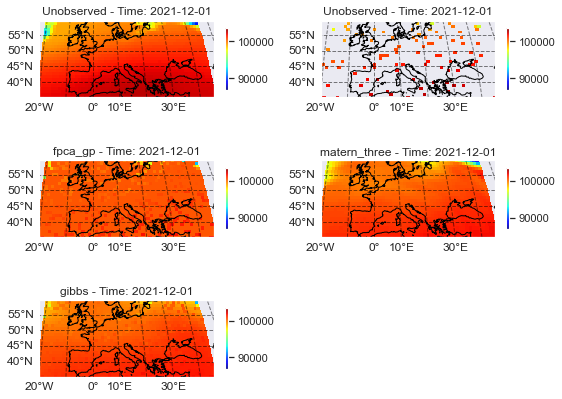
\includegraphics[width=\textwidth]{full_ex_ps_eur}
	\caption{An indicative example of the CPACE model performance on reconstruction for the European study of the CESM-LE PS variable using the various models in the European study. Clockwise from the top left we have the true data, the observed data at a particular time point, the Mat\'ern Three model reconstruction, the Gibbs model reconstruction, and the PACE model reconstruction under the CPACE framework.}
	\label{fig:full_ex_ps_eur}
\end{figure}

\subsection{Temperature \label{ssec:cesm_trefht_eur}}
In this section we present the results of the European study for the temperature variable. 
Alike Section~\ref{ssec:cesm_ps_eur}, we begin by considering the eigen decompostion of the data set which is common to all models under the PACE and CPACE frameworks. 

Figure~\ref{fig:phi_trefht_eur} shows the impact of the leading two eigenfunction in the decomposition for an example simulation. 
Similar to the pressure variable, the first eigenfunction is clearly a level shift of the mean function, with the second being a stretching of the peaks and troughs.
Again, this is encouraging, as they are intuitively reasonable leading modes of variation. 
It is reasonable to assume that as we move south the contribution of the first will be to shift the mean function higher to represent the effect of lower latitude on the overall temperature across time.

\begin{figure}
	\centering
	\begin{subfigure}[b]{0.45\textwidth}
		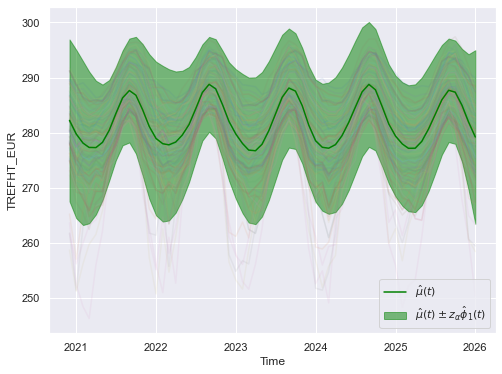
\includegraphics[width=\textwidth]{phi_1_trefht_eur}
		\caption{First eigenfunction.}
		\label{fig:phi_1_trefht_eur}
	\end{subfigure}
	\hfill        
	\begin{subfigure}[b]{0.45\textwidth}
		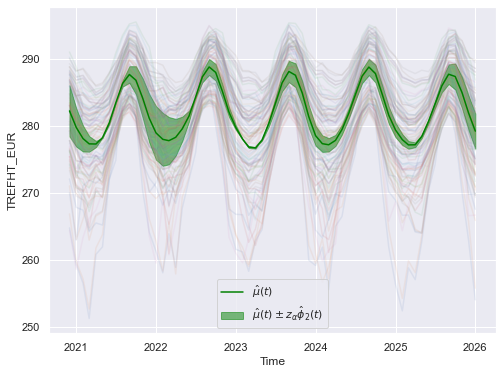
\includegraphics[width=\textwidth]{phi_2_trefht_eur}
		\caption{Second eigenfunction.}
		\label{fig:phi_2_trefht_eur}
	\end{subfigure}
	\caption{The first two eigenfunctions impact on the mean function from the PACE and CPACE framework for the TREFHT variable in the European study. Here the shaded region shows the impact of two standard deviations from the mean function using the corresponding eigenfunction. Sample curves from the dataset are plotted for context.}
	\label{fig:phi_trefht_eur}
\end{figure}

We now move on to consider how the models perform on the validation data.
Table~\ref{tab:train_cesm_trefht_eur} present these results.
We see similar results for all models, and there is only slight noticeable improvements from the spatial kernels.
This is expected as the PACE and CPACE methodology will utilise the observed values to inform the predicted function.
It so happens in this study that the CPACE models don't gain much additional information from neighbouring curves. 

\begin{table}
	\caption[Results for TREFHT variable on validation data in the European study]{Results for reconstruction of the validation data for the TREFHT variable in the European study from the CESM-LE dataset. Bold indicates best in class.}
	\centering
	\label{tab:train_cesm_trefht_eur}
	\begin{tabular}{lcc}
		\toprule
		\textbf{Model} & \textbf{RMSE} & \textbf{MAE} \\
		\midrule
		\verb*|pace| & 1.7037 (0.0817) & 1.0890	(0.0586) \\
		\verb*|fpca_gp| & 1.6692 (0.0653) & 1.0855	(0.0464) \\
		\verb*|matern_three| & \textbf{1.6115 (0.0767)} & \textbf{1.0348	(0.0593)}\\
		\verb*|gibbs| & 1.6522	(0.0865) & 1.0662 (0.0552)\\
		\bottomrule
	\end{tabular}
\end{table}

We now consider the comparative performance on the test set.
Here we may expect that utilising spatial information will give a good performance boost to the CPACE framework with spatial kernels.
Table~\ref{tab:test_cesm_trefht_eur} displays these results.

In fact we do see such an improvement, which again is an encouraging sign that the CPACE framework is applicable to this smaller spatial scale of the European study.
As an illustrative example we display a reconstruction for a test curve from this dataset in Figure~\ref{fig:test_ex_trefht_eur}.
It is interesting to note here, that the confidence interval for the Gibbs kernel is much more appropriate than the Mat\'ern model. 
This might suggest that while the Mat\'ern model performs best in mean, the Gibbs model actually predicts with a more realistic confidence interval. 


\begin{table}
	\caption[Results for TREFHT variable on test data in the European study]{Results for reconstruction of the test data for the TREFHT variable in the European study from the CESM-LE dataset. Bold indicates best in class.}
	\centering
	\label{tab:test_cesm_trefht_eur}
	\begin{tabular}{lcc}
		\toprule
		\textbf{Model} & \textbf{RMSE} & \textbf{MAE} \\
		\midrule
		\verb*|pace| &5.0376 (0.1367) & 3.9641	(0.1143) \\
		\verb*|fpca_gp| & 	5.0376	(0.1367) & 3.9641 (0.1143) \\
		\verb*|matern_three| & \textbf{	1.7362 (0.0671)} & \textbf{1.0726 (0.0228)}\\
		\verb*|gibbs| & 1.9959 (0.0535) & 1.2047 (0.0456)\\
		\bottomrule
	\end{tabular}
\end{table}

\begin{figure}
	\centering
	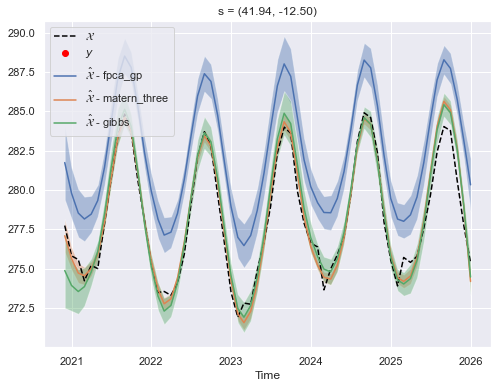
\includegraphics[width=\textwidth]{test_ex_trefht_eur}
	\caption{Example reconstruction for unobserved curves between our studied models for the TREFHT variable in the European study.}
	\label{fig:test_ex_trefht_eur}
\end{figure}

Next we compare the results for full reconstruction of the dataset using our image reconstruction metrics.
These are displayed in Table~\ref{tab:full_cesm_trefht_eur}.
Again we see the Mat\'ern model performing best in class, but in fact the Gibbs and Mat\'ern model perform similarly.
We note, as expected, a good improvement over the PACE framework using spatial dependent kernels.
An illustration of the effect is given in Figure~\ref{fig:full_ex_trefht_eur}.
We see good reconstruction overall in this example, but unfortunately all models fail to capture the more extreme areas of the study, such as the most north-westerly locations.
The spatial kernels tend to over smooth this area and therefore under predict the values of the data in this location.
We might expect the Gibbs kernel to be able to predict such spatial variation, however it seems in this study that the Gibbs model prefers to closely align with the Mat\'ern model.
We reason this will be because there is insufficient evidence in the training data to suggest such non-stationary dependency. 

\begin{table}
	\caption[Results for TREFHT variable on full data in the European study]{Results for reconstruction of the full data for the TREFHT variable in the European study from the CESM-LE dataset. Bold indicates best in class.}
	\centering
	\label{tab:full_cesm_trefht_eur}
	\begin{tabular}{lcc}
		\toprule
		\textbf{Model} & \textbf{PSNR} & \textbf{SSIM} \\
		\midrule
		\verb*|pace| & 15.3612	(0.1563)& 0.3402 (0.0046) \\
		\verb*|fpca_gp| & 15.3692 (0.1543)& 0.3426	(0.0072) \\
		\verb*|matern_three| & \textbf{24.1329	(0.1560)}& \textbf{0.9188 (0.0035)}\\
		\verb*|gibbs| & 23.0612	(0.1784) & 0.8957 (0.0047)\\
		\bottomrule
	\end{tabular}
\end{table}

\begin{figure}
	\centering
	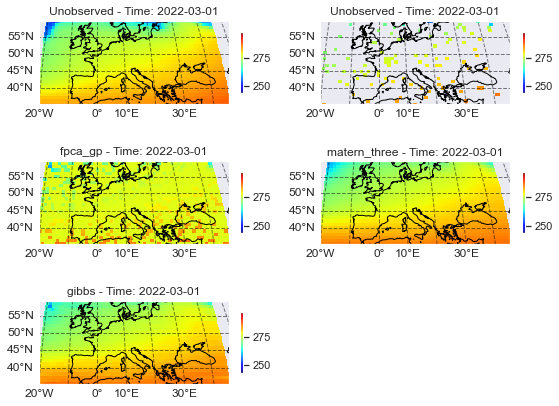
\includegraphics[width=\textwidth]{full_ex_trefht_eur}
	\caption{An indicative example of the CPACE model performance on reconstruction for the European study of the CESM-LE TREFHT variable using the various models in the European study. Clockwise from the top left we have the true data, the observed data at a particular time point, the Mat\'ern Three model reconstruction, the Gibbs model reconstruction, and the PACE model reconstruction under the CPACE framework.}
	\label{fig:full_ex_trefht_eur}
\end{figure}

\subsection{Precipitation \label{ssec:cesm_tmq_eur}}
In this section we present the results of the European study for the Precipitation variable. 
Alike Section~\ref{ssec:cesm_trefht_eur}, we begin by considering the eigen decompostion of the data set which is common to all models under the PACE and CPACE frameworks.

As with the study of other variables we display the first two eigenfunctions impact on the estimate mean function for the TMQ variable.
This can be seen in Figure~\ref{fig:phi_tmq_eur}.
Two things are displayed in this.

First, compared to the global study of the same variable in Section~\ref{ssec:cesm_tmq}, we see a stronger estimation of the mean function.
That is for two reasons.
The density of observations over space and frequency of observations across time is higher in the European study compared to the global study, by construction.
By nature of the mean estimator we have used, described in Section~\ref{sec:cpace_mean_estim} and Theorem~\ref{thm:cpace_mean}, we will converge to the true mean given more observations.
We also have, that the variability across space is less in the European study than that of the global study.
This means that functions tend to be closer to the mean function, and so our estimate is often less skewed by unusual functions in this study.
One important point is that in the global study we will tend to have two sets of functions with alternate periods.
These correspond to the functions from the two hemispheres of the globe respectively.
This added variability is not present in the European study.

Second, in addition to the level shift of the first eigenfunction, in Figure~\ref{fig:phi_1_tmq_globe}, the second eigenfunction captures the variability in the peaks and troughs.
This is similar to the other European studies.
Again this provides confidence in the PACE and CPACE methodologies as they seem to pull out natural eigenfunctions.

\begin{figure}
	\centering
	\begin{subfigure}[b]{0.45\textwidth}
		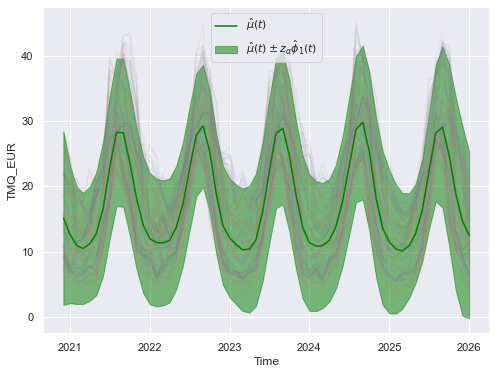
\includegraphics[width=\textwidth]{phi_1_tmq_eur}
		\caption{First eigenfunction.}
		\label{fig:phi_1_tmq_eur}
	\end{subfigure}
	\hfill        
	\begin{subfigure}[b]{0.45\textwidth}
		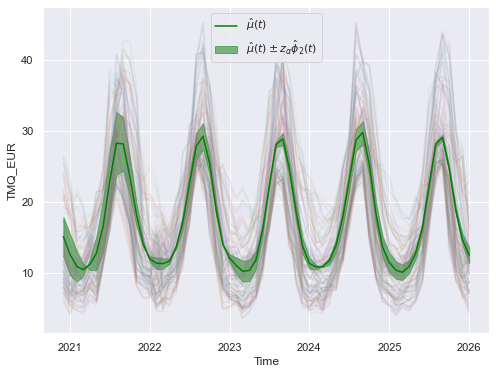
\includegraphics[width=\textwidth]{phi_2_tmq_eur}
		\caption{Second eigenfunction.}
		\label{fig:phi_2_tmq_eur}
	\end{subfigure}
	\caption{The first two eigenfunctions impact on the mean function from the PACE and CPACE decomposition framework for the TMQ variable in the European study. Here the shaded region shows the impact of two standard deviations from the mean function using the corresponding eigenfunction. Sample curves from the dataset are plotted for context.}
	\label{fig:phi_tmq_eur}
\end{figure}

Next we summarise the various models ability to reconstruct the validation data set.
This is given in Table~\ref{tab:train_cesm_tmq_eur}.
As can be seen, and alike other variable for the European study, both the PACE and CPACE models perform comparatively.
The distribution of these metrics is displayed in Figure~\ref{fig:cesm_tmq_eur_dist}, which highlights why we have chosen the Mat\'ern kernel as best in class.
This is encouraging from the CPACE models, since it highlights we do not loose any predictive ability using this Gaussian Process framework.
Equally, the same reasoning applies as to why we dont see much improvement using the spatial kernels from the other European studies, namely the added density of observations means each function with partially observed data is more well observed meaning the models lean towards using this information to aid in predictions.
Thus the spatial models gain less of a bonus from incorporating this additional spatial information.
It is reassuring to see from this that the spatial kernels aren't becoming overly confident on the spatial component of the modelling.
This can occur due to numerical issues when estimating the hyper parameters of the spatial kernels which cause the spatial kernel to essentially neglect the fact that the temporal component is present, by making them exceedingly large.
This is discussed more in Chapter~\ref{cha:implementation}.

\begin{table}
	\caption[Results for TMQ variable on validation data in the European study]{Results for reconstruction of the validation data for the TMQ variable in the European study from the CESM-LE dataset. Bold indicates best in class.}
	\centering
	\label{tab:train_cesm_tmq_eur}
	\begin{tabular}{lcc}
		\toprule
		\textbf{Model} & \textbf{RMSE} & \textbf{MAE} \\
		\midrule
		\verb*|pace| & 2.5156 (0.0615) & 1.8872	(0.0402) \\
		\verb*|fpca_gp| & 2.5206 (0.0614) & 1.8905 (0.0393) \\
		\verb*|matern_three| & \textbf{2.3960 (0.0561)} & \textbf{1.7995 (0.0446)}\\
		\verb*|gibbs| & 2.4649 (0.0663) & 1.8489 (0.0426)\\
		\bottomrule
	\end{tabular}
\end{table}


\begin{figure}
	\centering
	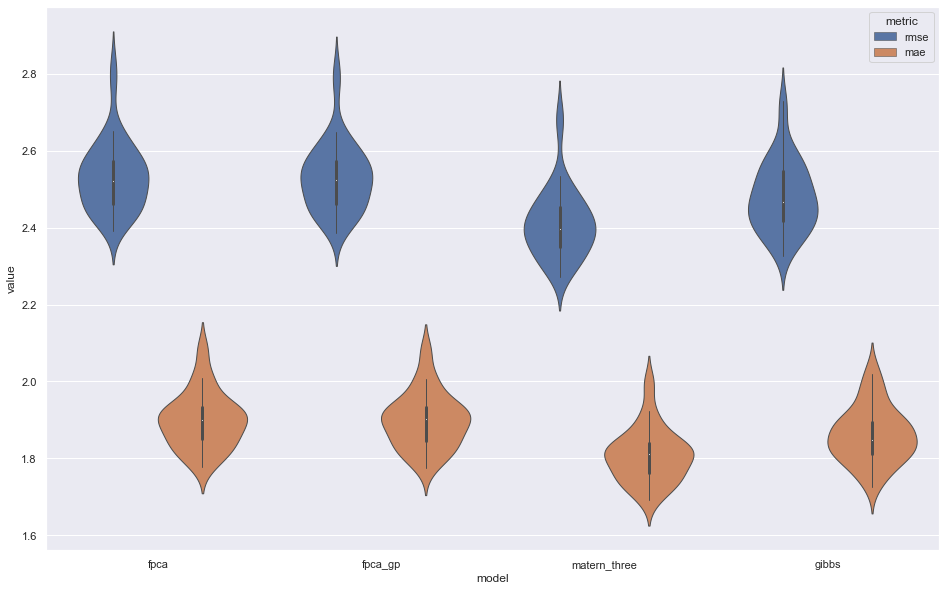
\includegraphics[width=\textwidth]{cesm_tmq_eur_dist}
	\caption{Distribution plot of the RMSE and MAE metrics on validation data for the TMQ variable in the European study.}
	\label{fig:cesm_tmq_eur_dist}
\end{figure}

Next we consider the performance of our models on the test dataset.
As mentioned in Section~\ref{ssec:eval_metrics}, this corresponds to functional data which we have not observed at all during estimation of model components and kernel hyper parameters where applicable.
Table~\ref{tab:test_cesm_tmq_eur} presents these results.

\begin{table}
	\caption[Results for TMQ variable on test data in the European study]{Results for reconstruction of the test data for the TMQ variable in the European study from the CESM-LE dataset. Bold indicates best in class.}
	\centering
	\label{tab:test_cesm_tmq_eur}
	\begin{tabular}{lcc}
		\toprule
		\textbf{Model} & \textbf{RMSE} & \textbf{MAE} \\
		\midrule
		\verb*|pace| & 5.0394 (0.0966) & 4.0714	(0.1078) \\
		\verb*|fpca_gp| & 5.0394 (0.0966) & 4.0714 (0.1078) \\
		\verb*|matern_three| & \textbf{2.4122 (0.0514)} & \textbf{1.8100 (0.0414)}\\
		\verb*|gibbs| & 2.5766 (0.0953) & 1.9292 (0.0670)\\
		\bottomrule
	\end{tabular}
\end{table}

Again, we see the Mat\'ern model being best in class.
Although the Gibbs model performs just as well, and both spatial kernels outperform the non-spatial models.
It is encouraging to see that the \verb*|pace| and \verb*|fpca_gp| model perform equally, as these models are theoretically equivalent as explained in Chapter~\ref{cha:cpace}.
This is a good indication that even on real world data sets using the CPACE framework is not detrimental to prediction performance in application.
For an illustration of the improvements the CPACE framework with spatial kernels can make, we display an example of a curve prediction across the whole temporal domain in Figure~\ref{fig:test_ex_tmq_eur}.
Here we can see clearly, how the spatial models are informed by the neighbouring observed curves to help firstly predict the level shift in the curves, but also help in predicting the amplitude shift to the mean function.
It is interesting to note how similar the Gibbs and Mat\'ern models predict here.
However, in this case the Gibbs model confidence band for the prediction seems much more reasonable, whereas the Mat\'ern model seems to be overly confident.

\begin{figure}
	\centering
	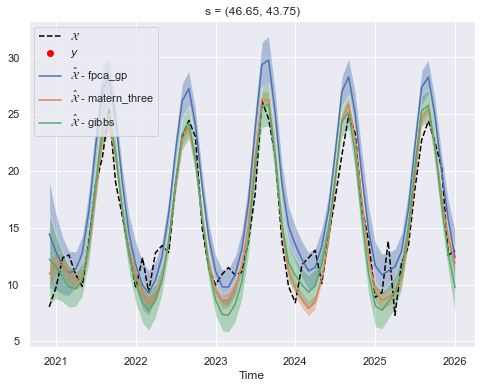
\includegraphics[width=\textwidth]{test_ex_tmq_eur}
	\caption{Example reconstruction for unobserved curves between our studied models for the TMQ variable for the European study.}
	\label{fig:test_ex_tmq_eur}
\end{figure}

Finally, we consider the image reconstruction metrics for the models.
Given the similar performance between the Gibbs and Mat\'ern models, as with other studies, the difference between image reconstruction metrics which consider perceived similarity between the true surfaces and the reconstruction may often be the metric of interest in choosing which to use for real world applications.
These metric results are given in Table~\ref{tab:full_cesm_tmq_eur}.
This confirms the Mat\'ern models best in class performance.
However, two other important points can be raised from this.
Firstly; the \verb*|fpca_gp| model performs slightly better in mean than the PACE model.
As seen with the simulation study in Section~\ref{sec:sim_summ}; this is due to  the ability to tune the kernel variances. 
Secondly; we see a slightly bigger variance of the Gibbs model results.
We look at what causes this for the SSIM metric in Figure~\ref{fig:full_tmq_eur_dist}, which considers the distribution of the SSIM metrics for this study between the Mat\'ern and Gibbs models.
We can see that while the Gibbs model performs worse on average, it occasionally performs better.
This indicates it might not be a clear cut decision that the Mat\'ern model is always the correct kernel to choose for this study.

\begin{table}
	\caption[Results for TMQ variable on full data in the European study]{Results for reconstruction of the full data for the TMQ variable in the European study from the CESM-LE dataset. Bold indicates best in class.}
	\centering
	\label{tab:full_cesm_tmq_eur}
	\begin{tabular}{lcc}
		\toprule
		\textbf{Model} & \textbf{PSNR} & \textbf{SSIM} \\
		\midrule
		\verb*|pace| & 14.3970 (0.1016) & 0.2674 (0.0068) \\
		\verb*|fpca_gp| & 14.3976 (0.1021) & 0.2679	(0.0064) \\
		\verb*|matern_three| & \textbf{20.5960 (0.2607)}& \textbf{0.7951 (0.0073)}\\
		\verb*|gibbs| & 19.9990	(0.3397)& 0.7650 (0.0168)\\
		\bottomrule
	\end{tabular}
\end{table}

\begin{figure}
	\centering
	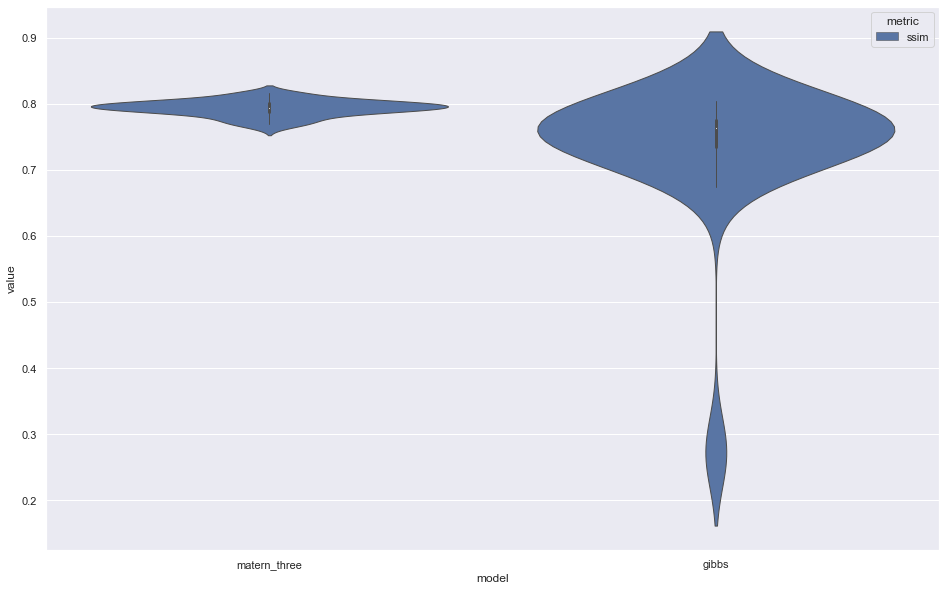
\includegraphics[width=\textwidth]{full_tmq_eur_dist}
	\caption{Distribution plot of the SSIM metric on full data for the TMQ variable in the European study for the Mat\'ern and Gibbs kernel.}
	\label{fig:full_tmq_eur_dist}
\end{figure}

Irrespective of this we can see clearly a performance increase in using the CPACE framework with spatial kernels.
Whilst this is not unexpected and ties in nicely with the global study and the simulation study, it is encouraging to see that the CPACE framework continues to outperform the PACE framework on  higher density observed functional data which is under consideration in this study.
Finally, for illustration we display an example reconstruction for all models for a specific point in time across the full spatial domain in Figure~\ref{fig:full_ex_tmq_eur}.
Here, we can clearly see the visual  improvements which are represented in the metrics throughout this section.
However, we can also see that there are some areas in which we just don't capture the spatial variation correctly.
These corresponds to the areas of the highest peaks  and troughs, where we fail to capture this extreme rapid variation from the mean curve completely.
This is likely because the spatial variation changes quite rapidly over time in this dataset.
The CPACE model assume separate but constant spatial structure over time for each eigenfunction, and so with our $5$ components in the models we do not capture these extreme cases of spatial variation, which occur infrequently over time.
Increasing the number of components in our models would likely alleviate this issue, however for this study we have not considered how to choose $K$ .
A discussion on this, not relating to these studies, is given in Chapter~\ref{cha:implementation}.
More modest variation across space is well captured however since this tends to be more consistent over time.

\begin{figure}
	\centering
	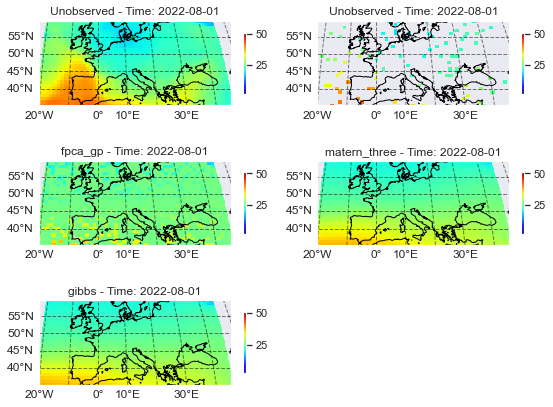
\includegraphics[width=\textwidth]{full_ex_tmq_eur}
	\caption{An indicative example of the CPACE model performance on reconstruction for the European study of the CESM-LE TMQ variable using the various models in the European study. Clockwise from the top left we have the true data, the observed data at a particular time point, the Mat\'ern Three model reconstruction, the Gibbs model reconstruction, and the PACE model reconstruction under the CPACE framework.}
	\label{fig:full_ex_tmq_eur}
\end{figure}

\subsection{Wind Speed \label{ssec:cesm_u10_eur}}
In this section we present the results of the European study for the Wind Speed variable. 
We begin by considering the training metrics for this study.
That is the RMSE and MAE for our models ability to reconstruct partially observed functions.
Table~\ref{tab:train_cesm_u10_eur} displays the mean and standard deviation of these metrics from the $40$ simulations which are part of the CESM-LE dataset. 
Again, as we have seen in the other European studies, all models perform equally well.
The Mate\'rn is chosen as best in class because of its lower mean metric scores.
However, all models are within one standard deviation of each other, hence this isn't a definitive indication that this kernel will perform best over all simulations.

Figure~\ref{fig:train_ex_u10_eur} gives an illustration of a reconstruction of partially observed function.
We can see that on the whole the models captures the periodic nature well, but struggle to capture the amplitude changes between observations.
This isn't an unusual sight for models with a periodic temporal component.
 
\begin{table}
	\caption[Results for U10 variable on validation data in the European study]{Results for reconstruction of the validation data for the U10 variable in the European study from the CESM-LE dataset. Bold indicates best in class.}
	\centering
	\label{tab:train_cesm_u10_eur}
	\begin{tabular}{lcc}
		\toprule
		\textbf{Model} & \textbf{RMSE} & \textbf{MAE} \\
		\midrule
		\verb*|pace| & 1.1300 (0.0374) & 0.8958	(0.0295) \\
		\verb*|fpca_gp| & 1.1277 (0.0375) & 0.8930 (0.0288) \\
		\verb*|matern_three| & \textbf{1.0906 (0.0351)} & \textbf{0.8642 (0.0273)}\\
		\verb*|gibbs| & 1.1130 (0.0381) & 0.8807	0.0281\\
		\bottomrule
	\end{tabular}
\end{table}

\begin{figure}
	\centering
	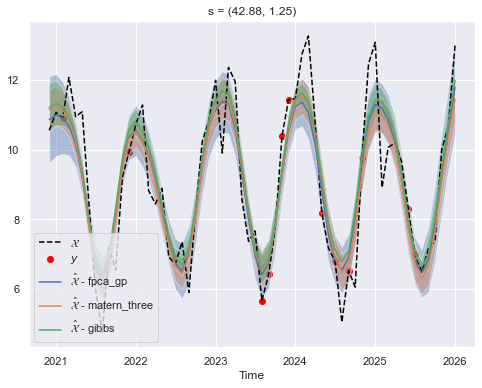
\includegraphics[width=\textwidth]{train_ex_u10_eur}
	\caption{Example reconstruction for partially observed curves between our studied models on the U10 variable of the CESM-LE dataset in the European study.}
	\label{fig:train_ex_u10_eur}
\end{figure}

A similar set of results is obtained by looking at the performance of the models on the test data, that is the prediction of completely unobserved functional data.
Table~\ref{tab:train_cesm_u10_eur} displays these results.
Here, we can clearly see a preference for the spatial kernels under the CPACE framework.
Unlike the European studies for the previous variables interest, the Mat\'ern model is clearly the best model for this variable.
An example reconstruction of a test data point is given in Figure~\ref{fig:test_ex_u10_eur} which highlights the difference between models. 
We can see clearly that they all fail to capture the variation in the peak in the middle of the domain, but the spatial kernel models capture the beginning and end of the temporal domain much better than the non-spatial kernel. 
The Mat\'ern model seems to slightly outperform the Gibbs kernel in this one example in this area also. 

\begin{table}
	\caption[Results for U10 variable on test data in the European study]{Results for reconstruction of the test data for the U10 variable in the European study from the CESM-LE dataset. Bold indicates best in class.}
	\centering
	\label{tab:test_cesm_u10_eur}
	\begin{tabular}{lcc}
		\toprule
		\textbf{Model} & \textbf{RMSE} & \textbf{MAE} \\
		\midrule
		\verb*|pace| & 1.6801 (0.0340) & 1.2104	(0.0276) \\
		\verb*|fpca_gp| & 1.6801 (0.0340) & 1.2104 (0.0276) \\
		\verb*|matern_three| & \textbf{1.1354 (0.0425)} & \textbf{0.8908 (0.0242)}\\
		\verb*|gibbs| & 1.3265 (0.0613) & 1.0053 (0.0299)\\
		\bottomrule
	\end{tabular}
\end{table}

\begin{figure}
	\centering
	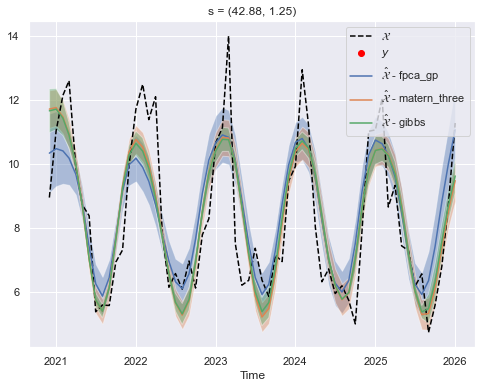
\includegraphics[width=\textwidth]{test_ex_u10_eur}
	\caption{Example reconstruction for unobserved curves between our studied models for the U10 variable for the European study.}
	\label{fig:test_ex_u10_eur}
\end{figure}

Finally, we consider the ability of the models under the image reconstruction metrics as described in Section~\ref{sec:cesm_study}.
We display these results in Table~\ref{tab:full_cesm_u10_eur}.
As expected we see the Mat\'ern model performing best in class.
However, it is interesting to note that unlike the the previous variables in the European study, the ability to reconstruct the U10 variable is much less.
We can see a clear example of the struggles of modelling this data through Figure~\ref{fig:full_ex_u10_eur}, which shows the reconstruction across the whole domain at a particular point in time.
Here, it is obvious all models missed the large increase in windspeed in the Atlantic.
Similar to the study on the precipitation, Section~\ref{ssec:cesm_tmq_eur}, this is because this phenomena is short lived, and the spatial variation is not constant through time.
The short lived nature of such phenomena make it difficult for the PACE and CPACE frameworks to pick up as eigenfunctions, since overall it doesn't account for much variation. 
Further, the change in spatial variation this causes is not picked up by the CPACE framework as it would be required to be an eigenfunction which would then get its own spatial variation over time. 
One way to capture this would be to let $K$, the number of components of the model be increased.
However, in these studies we have not considered how to choose $K$, a discussion on this is presented in Chapter~\ref{cha:implementation}.

\begin{table}
	\caption[Results for U10 variable on full data in the European study]{Results for reconstruction of the full data for the U10 variable in the European study from the CESM-LE dataset. Bold indicates best in class.}
	\centering
	\label{tab:full_cesm_u10_eur}
	\begin{tabular}{lcc}
		\toprule
		\textbf{Model} & \textbf{PSNR} & \textbf{SSIM} \\
		\midrule
		\verb*|pace| & 15.7694 (0.1047) & 0.2681 (0.0034) \\
		\verb*|fpca_gp| & 15.7721 (0.1054) & 0.2688	(0.0033)\\
		\verb*|matern_three| & \textbf{18.7107	(0.1809)}& \textbf{0.4674 (0.0139)}\\
		\verb*|gibbs| & 17.5800	(0.3304)& 0.4257 (0.0173)\\
		\bottomrule
	\end{tabular}
\end{table}

\begin{figure}
	\centering
	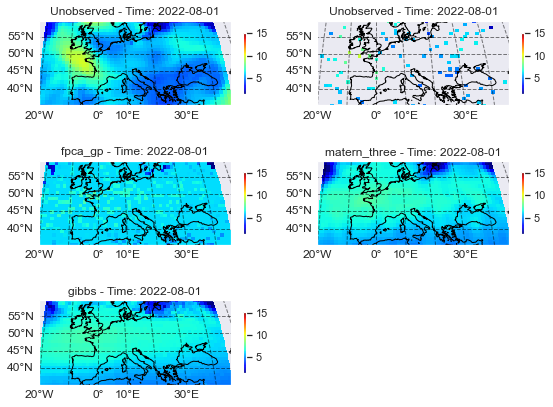
\includegraphics[width=\textwidth]{full_ex_u10_eur}
	\caption{An indicative example of the CPACE model performance on reconstruction for the European study of the CESM-LE U10 variable using the various models. Clockwise from the top left we have the true data, the observed data at a particular time point, the Mat\'ern Three model reconstruction, the Gibbs model reconstruction, and the PACE model reconstruction under the CPACE framework.}
	\label{fig:full_ex_u10_eur}
\end{figure}

It is also interesting to note, that in Figure~\ref{fig:full_ex_u10_eur}, we can see the Gibbs kernel and the Mat\'ern kernel disagreeing on the structure.
One example is the area over the Baltic sea;  where the Gibbs model prefers a more variable structure here than the Mat\'ern kernel.
This is a prime example of the added flexibility of the non-stationary Gibbs kernel. 

\subsection{Discussion \label{ssec:cesm_dis_eur}}
In the above, we have considered comparing the PACE methodology with our CPACE framework with a number of different kernel on a subset of the full CESM-LE dataset.
We can see that in all cases, alike with the global studies, the CPACE spatially dependent models outperform the PACE framework.
This is again intuitive due to the geographic nature of the dataset clearly has a spatial component that isn't present in a PACE framework.

Our results suggest a Mat\'ern kernel is typically the most appropriate kernel of the three considered.
This is usually closely followed by the Gibbs kernel, and in some cases the Gibbs Kernel is preferred, especially when considering the model which may maximise the image reconstruction metrics.
We can see a clear improvement in reconstructing the smaller European dataset than compared to the global study.
Again, this is quite expected due to the construction of this study having denser observations.
This allows for a better estimate of the  mean and covariance structure, which are used in both the PACE and CPACE framework.
It is encouraging to note that the CPACE framework still outperforms the PACE framework in this setting, that is the denser observations do not reduce the need for a spatial kernel.
Although we do see a slight decrease in comparative performance of the CPACE framework on partially observed functions when densely observed.

The wind speed, U10, and precipitation, TMQ, in general were the most difficult to model.
As explained in Sections~\ref{ssec:cesm_u10_eur},~\ref{ssec:cesm_tmq_eur} respectively this is because of non-constant spatial variation over time, and the limited number of component eigenfunctions we have used in this study.

The European studies illustrate that the CPACE framework is quite applicable to smaller spatial scale studies.


\section{Summary \label{sec:cesm_summ}}
In the above global and european studies, Sections~\ref{sec:cesm_res},~\ref{sec:cesm_res_eurr} respectively, we compared how the CPACE framework handles our CESM-LE data.
As described in Section~\ref{sec:cesmle}, this is often used as a real world  EO data set.
The data generating process of this dataset is far removed from the assumed model that the CPACE framework is based on.
We see encouraging results from both studies.
Noticing a good performance increase on the pixel related metrics of the RMSE and MAE.
More importantly for application perhaps, we notice a good increase in the SSIM and PSNR for the spatially dependent CPACE models.
This indicates these models are ideal candidates to help reproduce imagery from partial or completely missing EO data to be used by a person.

We have explored the difference the CPACE framework makes on both densely observed data, as in the European study, and on very sparsely observed data in the Global study.
The improvements seen using the same framework in both is encouraging, and as discussed in Chapter~\ref{cha:implementation}, the setup  and implementation for various spatial domains requires little fine tuning.

We note that improvements from the PACE methodology was seen across all variables of interest, however all models found the U10 and TMQ datasets most difficult to predict.
This we reasoned is due to these variables having the most complicated generating procedure, with examples of spatial variation which is non-constant through time.
This is something which would require a complete eigenfunction and the corresponding spatial kernel to capture in the CPACE model and we studied models with a fixed $5$ components which typically wasn't enough to capture this independently. 
The reasoning on how to select $K$, the number of components in the CPACE model, is briefly discussed in Chapter~~\ref{cha:implementation} and is not something we considered for these studies.

It is notable, that in the eigen decomposition of all the variables, across the European and global studies, the first eigenfunction typically related to a level shift of the mean function.
This is both interesting and encouraging, as this often corresponds to a shift in the mean function as you travel across latitude bands of the globe.
This highlights an important aspect of the PACE modellingl; which is its ability to explain data sets.
This is something that the CPACE framework keeps with the same eigen decomposition. 
It is encouraging to see that this application resulted in such interpretable eigenfunctions.